
\def\g4{{\sf Geant4}}

\newcommand{\codeAlgorithm}[1]{
\addcontentsline{toc}{section}{Résumé}
\begin{center}\fbox{\parbox{12cm}{\bf #1}}\end{center}}

\newcommand{\cppintro}[1]{
\lstset{language=C,
caption= #1 ,
label=listing:boundary}}

\def\cppstart{\begin{lstlisting}}
\def\cppend{\end{lstlisting}}%% Uncomment these if you write in English

\documentclass[12pt]{article}
\usepackage[english]{thesis}

\usepackage[utf8]{inputenc} % look here if scands are broken

%% Jos käytät latex-komentoa käännettäessä (oletusarvo) 
%% kuvat kannattaa tehdä eps-muotoon. Älä käytä ps-muotoisia kuvia!
%% Käytä seuraavaa latex-komennon ja eps-kuvien kanssa 
%%\usepackage[dvips]{graphicx}

%% Jos tääs käytät pdflatex-komentoa, 
%% joka kääntää tekstin suoraan pdf-tiedostoksi ja kuvasi
%% ovat esim. jpg-formaatissa tai pdf-formaatissa,   
%% käytetään seuraavaa pakettia, kommentoi siis kommenttimerkki pois
%% Huom! Tekstin marginaalit saattavat poiketa n. 2-5 mm
%% suosituksesta, jos käytät pdflatex-komentoa!
\usepackage[pdftex]{graphicx} 
\usepackage{multirow}
\usepackage{url}
\usepackage{listings}
%\usepackage{graphicx}
\usepackage[utf8]{inputenc} % look here if scands are broken
\usepackage{wrapfig}
%\usepackage{makeidx}
%\usepackage{subfig}
\usepackage{fancyhdr}
%\usepackage{asymptote}
\usepackage{amsmath}
\usepackage{verbatim} % for comment
\usepackage{eurosym} 
\usepackage{color} % for definecolor
\usepackage[colorlinks,bookmarks=true]{hyperref}
\usepackage{wasysym} %provides permille sign

%% Saat pdf-tiedoston viittaukset ja linkit kuntoon seuraavalla paketilla.
%% Paketti toimii erityisen hyvin pdflatexin kanssa. 
%\usepackage[pdfpagemode=None,colorlinks=true,urlcolor=red,%
%linkcolor=blue,citecolor=black,pdfstartview=FitH]{hyperref}

%% Jos et jostain syystä tykkää käyttää
%% edellistä hyperref pakettia, voit käyttää myös seuraavaa pakettia
%% (tarvitaan lähinnä url-komennon määrittämiseen ja formatoimiseen)
\usepackage{url}

%% Matematiikan fontteja, symboleja ja muotoiluja lisää, näitä tarvitaan usein 
\usepackage{amsfonts,amssymb,amsbsy}  
%% paketti että saa ladottua monta kuvaa samalle sivulle.
\usepackage{subfigure}

%% Käytä seuraavaa pakettia jos haluat
%% Times-fontit LaTeX:n normaalien Computer Modern-fonttien sijaan.
%% Times-fontit ja Computer Modern-fontit ovat kummatkin roomalaisia
%% fonttityyppejä ja monet kutsuvat kaikkia roomalaisia
%% fontteja virheellisesti Times-fonteiksi,
%% vaikka tarkasti ottaen Times on vain Times-lehden fontti.
%% Computer Modern on Donald Knuthin suunnittelema fontti, joka
%% on Century Magazinen fontin variantti.
%% Huom! Kaavoihin ei tule Times-fontteja, joten lopputulos ei ole
%% välttämättä aivan tyylikäs. Pakettia ei suositella sen vuoksi. 
%\usepackage{times}  

%% Vaakasuunnan mitat, ÄLÄ KOSKE!
\setlength{\hoffset}{-1in}
\setlength{\oddsidemargin}{35mm}
\setlength{\evensidemargin}{25mm}
\setlength{\textwidth}{15cm}
%% Pystysuunnan mitat, ÄLÄ KOSKE!
\setlength{\voffset}{-1in}
\setlength{\headsep}{7mm}
\setlength{\headheight}{1em}
\setlength{\topmargin}{25mm-\headheight-\headsep}
\setlength{\textheight}{23cm}
%% Vasensuora-asettelu, joka opinnäytteessä vaaditaan. ÄLÄ KOSKE
\setlength{\parindent}{0pt}
\setlength{\parskip}{1ex}


%% Kaikki mikä paperille tulostuu, on tämän jälkeen
\begin{document}

\Language{English}{Englanti}

\university{helsinki university of technology}{teknillinen korkeakoulu}

%% Korjaa seuraavat vastaamaan omaa tiedekuntaasi
\faculty{Faculty of Information and Natural Sciences}%
{}%
%%

%% Vain kandityölle: Korjaa seuraavat vastaamaan tutkinto-ohjelmaasi
\degreeprogram{Engineering Physics and Mathematics}{}
%%

%% Vain DI- ja lisensiaatintyölle
%\professorship{Circuit theory}{Piiriteoria}
%\code{S-55}
%%

%% Valitse yksi näistä kolmesta
\degree{BSc}
%\degree{MSc}
%\degree{Lic}

%% Oma nimi
\author{Gillis Danielsen}

%% Opinnäytteen nimi tulee vain tähän
\thesistitle{Simulating carbon beam fragmentation on water phantom with Geant4}{}

%% Kandidaatintyön päivämäärä on sen esityspäivämäärä! 
%%\date{22.1.2008}

%% Kandidaattiseminaarin vastuuopettaja
\supervisor{Prof. Harri Ehtamo, Ph.D Veikko Karimäki}{}

%% Kandidaatintyön ohjaaja
\instructor{Ph.D Aatos Heikkinen}{}

%% Tehdään kansilehti
\makecoverpage

%% Tiivistelmän avainsanat 
\keywords{Geant4, Binary cascade, CERN, IAEA evaluation, Hadrontherapy, Bragg peak, fragment buildup}
%% Tiivistelmän tekstiosa
\begin{abstractpage}[english]
This thesis focuses on the simulation of carbon beams in a water phantom using Geant4 code. This study inspects the feasibility of Monte Carlo simulations for medical heavy-ion therapy. Geant4 is a multi-purpose physics simulation package developed at the European Organization for Nuclear Research (CERN). Geant4 gives the choice of multiple models suitable for the experiment, however, this paper focuses on the Binary model developed as a collaboration of scientists at CERN and other research institutions worldwide. Results are compared to experimental data made available at GSI Darmstadt by E.Haettner in 2006. Our work is part of the International Atomic Energy Agency (IAEA) coordinated programme to compile and evaluate charged-particle nuclear data and related Monte Carlo codes for therapeutic applications. We have introduced extensions to the Geant4 Hadrontherapy-example. Furthermore we have modeled and estimated especially the magnitude and distribution of fragment build-up at the end of the Bragg-curve.
\end{abstractpage}

%% Pakotetaan uusi sivu varmuuden vuoksi, jotta 
%% mahdollinen suomenkielinen ja englanninkielinen tiivistelmä
%% eivät tule vahingossakaan samalle sivulle
\newpage



%% Sisällysluettelo
%% addcontentsline tekee pdf-tiedostoon viitteen sisällysluetteloa varten
\addcontentsline{toc}{section}{Contents}
%% Tehdään sisällysluettelo
\tableofcontents


%% Symbolit ja lyhenteet
%\mysection{Symbols and legends}
%
%\begin{tabular}{ll}
%CERN         & Organisation europeenne pour la researche nucleare \\
%INCL      & intranuclear cascade, liege\\
%ABLA        & Abla \\tion Abration model\\
%IAEA         & International Atomic Energy Association \\
%HIP        & Helsinki Institute of Physics
%\end{tabular}


%% Sivulaskurin viilausta opinnäytteen vaatimusten mukaan:
%% Aloitetaan sivunumerointi arabialaisilla numeroilla (ja jätetään
%% leipätekstin ensimmäinen sivu tyhjäksi, 
%% ks. alla \thispagestyle{empty}).
%% Pakotetaan lisäksi ensimmäinen varsinainen tekstisivu alkamaan 
%% uudelta sivulta clearpage-komennolla. 
%% clearpage on melkein samanlainen kuin newpage, mutta 
%% flushaa myös LaTeX:n floatit 
\clearpage
\section{Acknowledgement}

This work was made as a part of the HIP summer student program at CERN in 2009. I would like to thank CERN and HIP for this incredible summer in a very scientific and innovative ambiance. I would also specifically like to thank the following persons for providing me with the help and support needed to accomplish this paper.

Firstly, I would like to thank my supervisor Ph.D Aatos Heikkinen for tireless efforts to make my stay at cern as productive and enjoyable as possible.

Ph.D Pekka Kaitaniemi of CEA was of great technical expertise and allways very helpfull in all issues.

I also greatly appreciate all the time M.Sc. Emma Haettner took to clarify through personal correspondance the unclear details involved in the data-sets recieved from GSI.

\cleardoublepage
\storeinipagenumber
\pagenumbering{arabic}
\setcounter{page}{1}


%% Ensimmäinen osa, LEIPÄTEKSTI ALKAA
\section{Introduction}
\thispagestyle{empty}
%Carbon beams are a promising new alternative to traditional radiation cancer therapy. 
The history of radiation treatments dates back to 1895 when W.K.~Roentgen discovered the x-rays. It was not long before these photon rays were used to treat malign tissue. The first methods used were on today's standards very crude, and much work has gone into perfecting the treatments in order to minimize the effect of the rays on the surrounding healthy tissue and maximize the dose delivered to the malign tissue.

However, due to the statistical nature of the photon interactions, a beam of many photons is
exponentially attenuated yielding an exponential decrease of the dose with the depth. To
obtain a higher dose in the tumor than in the surrounding normal tissue, many irradiation
fields are used. The cost of this method is that a large volume of the normal tissue
will suffer from a high dose. By replacing the x-rays with high energy photons, the dose
maximum is shifted a few centimeters deeper and the exponential decrease is more shallow,
which improves the ratio between dose in the tumors and in the normal tissue. Although very sophisticated variations of the photon treatments have been perfected over time, photon therapies still produce considerable harm to the surrounding tissue. 

Much younger and less widely used technologies are those of hadron- or heavy-ion based radiotherapies. Hadrons and heavier ions are charged particles and therefore interact with tissue in a much different way to photons. The dose-profile contains a much sharper peak due to the primary halting force being electromagnetic interaction. This peak is called the Bragg-peak, and was first discovered by William Henry Bragg in 1903.

The field of hadron treatments was pioneered at the Lawrence Berkeley Laboratory (LBL). Based on research done at the Berkeley cyclotron J.~Wilson first recommended the use of protons as a treatment method in a 1946 paper~\cite{RW46}. Furthermore, the first de facto treatment was administered at Berkeley in 1953. Today there are a number of proton-based therapies in clinical use all around the world, for example in Harvard General Hospital (see fig). %fixme
\begin{figure}[h]
\begin{center}
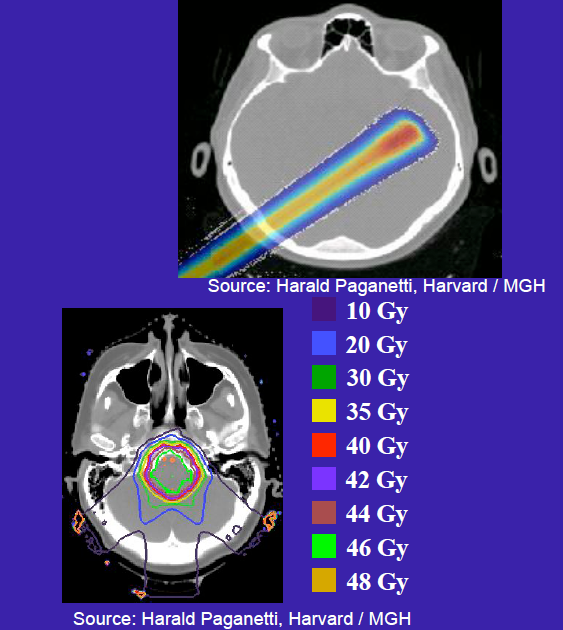
\includegraphics[width=0.75\textwidth]{images/HarvardHadronTreatment.png}  
\caption{\label{fig:HarvardHadron} Example of Geant4 proton treatment planing simulation for brain tumour shown.} 
\end{center}
\end{figure} 
Heavy-ion therapies have remained considerably less common and have remained on a more experimental level. Clinical trials were conducted at LBL inbetween 1977 and 1993 with $^{20}$Ne. At the end of 2008 the Particle Therapy Co-Operative  Group (PTCOG) estimated that more than 7000 heavy-ion treatments had been conducted at treatment facilities it monitors worldwide. Treatments based on $^{12}$C beams have been offered at NISR in Japan and in Germany at GSI~\cite{PTCOGstat}. Carbon beams is currently the most active and promising area of heavy-ion therapy research. 

The motivations for heavy-ion treatments as an alternative or complement to hadron treatments are considerable. Firstly carbon ions have the added advantage of higher ionization-density at the end of their range, causing greater correlated damage to the DNA-structure of a single cancerous cell and therefore induces damage in a way that makes it less likely the cell is able to repair. In a 2008 article O.~Jäkel~\cite{ojakel} approximates the beam's increase in biological efficiency by a factor between 1.5 and 3 in comparison to proton treatment depending on the application. Secondly, Heavy-ions ions are less scattered in lateral directions which yields better dosage control in many applications. However, the tradeoff is that carbon-ions will fragment into smaller particles, yielding an unwanted ``tail`` to the energy-loss profile. One of the main motivations of the work is to study this ''tail'' for the ``worst case scenario'' of 400~MeV, which is an upper limit in medical applications.

A number of data-sets are available for carbon beams. For this paper we choose to use experimental data made available by E.~Haettner as a part of her Master's thesis~\cite{ehaettner} at the Gesellschaft für Schwerionenforschung (GSI) facility in Darmstadt, Germany. This works reproduces the experimental setup used by E.Haettner as modelled in a simulation. The aim of this paper is to provide good reference data for the standardization work involved in hadron treatment. Furthermore, this paper evaluates the feasibility of the Geant4 models for such simulations by comparison to experimental data. This benchmarking is part of IAEA's INDC International Nuclear Data Committee and Heavy Charged-Particle Interaction Data For Radiotherapy project which compares different Monte Carlo codes~\cite{SummaryReport}.

%footnotta förkortningar?

\footnote{Bachelor's thesis produced in the framework of the Finnish CERN Summer Training 2009. Supervisors A.~Heikkinen and V.~Karimäki from Helsinki Institute of Physics and H.~Ehtamo of Helsinki University of Technology} %fixme footnote

%% Opinnäytteessä jokainen osa alkaa uudelta sivulta, joten clearpage
\clearpage
\section{Theory}

\subsection{Electromagnetic physics of Bragg-curve}
As charged particles penetrate tissue they interact with the tissue through elastic and inelastic collisions with the electrons and nuclei, eventually loosing all of their energy. The most typical interaction is that of inelastic collisions with electrons, contributing as much as 99\% of the total energy loss.

The beam's energy loss $dE/dx$ as a function of depth is described by the Bragg curve. %fixme see fig here
 Theoretical estimates for this relation have existed since the first classical treatment by Bohr in 1913~\cite{bohr13}. The currently used quantum model was derived by Bethe and Bloch in 1953~\cite{bethebloch53}  and is commonly known as "Bethe's stopping power formula". The Bethe stopping power formula is considered a good model for most fast charged particles, with the exception of electrons.

\begin{equation}
 \frac{dE}{dx} = \frac{4 \pi}{m_e c^2} \cdot \frac{nZ^2}{\beta^2} \cdot \left(\frac{e^2}{4\pi\varepsilon_0}\right)^2 \cdot \left[\ln \left(\frac{2m_e c^2 \beta^2}{I \cdot (1-\beta^2)}\right) - \beta^2\right],
\label{bethebloch}
\end{equation}
where $\beta = v/c $, 
$v$ is the velocity of the particle,
$E$ is the 
energy of the particle,
$x$ is the 
distance travelled by the particle,
$c$ is the 
speed of light,
$Z$ is the 
particle charge,
$e$ is the 
charge of the electron,
$m_e$ is the 
rest mass of the electron,
$n$ is the 
electron density of the target and 
$I$  is the 
mean excitation potential of the target.


However, as the speed of the particle has decreased to the order of magnitude of the Bohr velocity the nuclear charge $Z$ will no longer remain constant and has to be approximated by the effective charge, given by the Barkas formula. $$Z_{eff} = Z(1-e^{-125 \beta Z})$$

In this theoretical model the form of the Bragg-peak can be visualized as the $1/v^2$ relation increases the energy-loss as speed decreases. However, the effective charge will decrease at an exponential rate, thus, converging the Bragg-curve.

Particles penetrating matter do not only deposit energy through inelastic electron collisions, they might as well be involved in nuclear reactions and fragmented. A common simple model for explaining this is called the abrasion-ablation model. In this model high energy projectiles can be described as particles that move on straight lines through the
target. From time to time a target nucleus lie on this line, thus causing a collision. Bullet
and target nucleons which overlap eachother in this model (~\ref{fig:ablationabration}) are called participants. The remaining parts of the projectile and target nucleus are called spectators. The momentum of the spectators in the projectile and target are only slightly affected by the collision. The participant nucleons form an excited entity, ``a fireball'', which fragments into separate light ions or single nucleons.
The Wilson-model~\cite[Chapter 27]{physicsManual} that is also provided in Geant4 features a physics model more reminiscent to this approach.
\begin{figure}[h]
\begin{center}
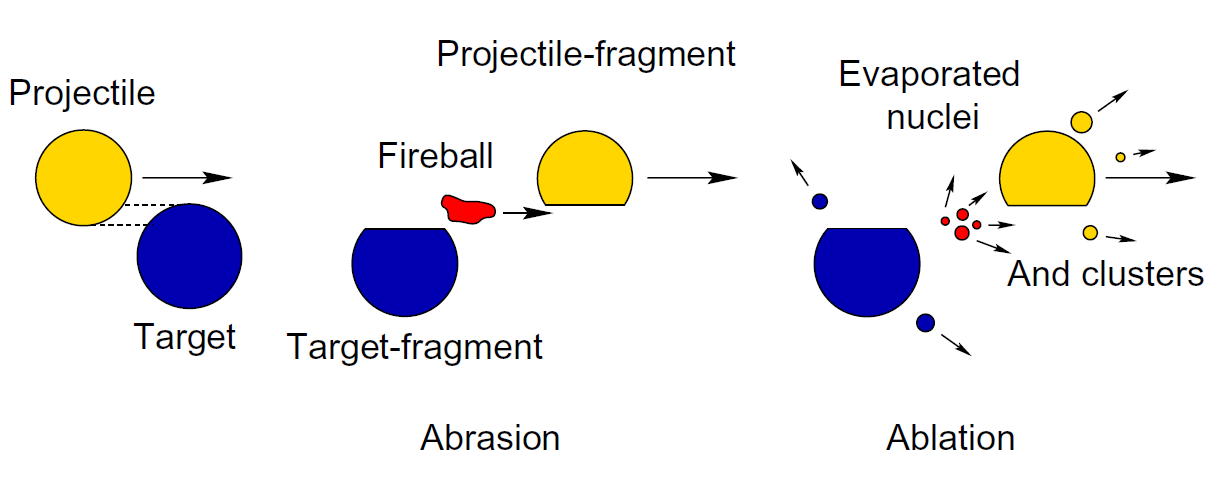
\includegraphics[width=0.8\textwidth]{images/ablationabration.png}  
\caption{Schematic description of the abrasion-ablation model in Geant4.~\cite[Chapter 27]{physicsManual}}
 \label{fig:ablationabration}
 \end{center}
 \end{figure}



\subsection{Theory of used models} %theory, no practical aspects

For this paper the models of interest are those involved in intranuclear interaction and thus in the production of new fragments. Geant4 moves particles around its geometry and according to defined stochastic relations determines when certain events take place by calling the appropriate models.

When a spallation process between two nuclei is determined to take place the Binary cascade model is called into action. The cascade model provides insight into the intranuclear processes that take place in the very short timeframe from the incident particle hitting the target particle. Once the immediate intranuclear interaction has taken place a much slower phase of evaporation and fission takes place. 

The evaporation phase is calculated by separate models that only need the excitation parameters of the nuclei left after the short cascading process.

\begin{figure}[h]
\begin{center}
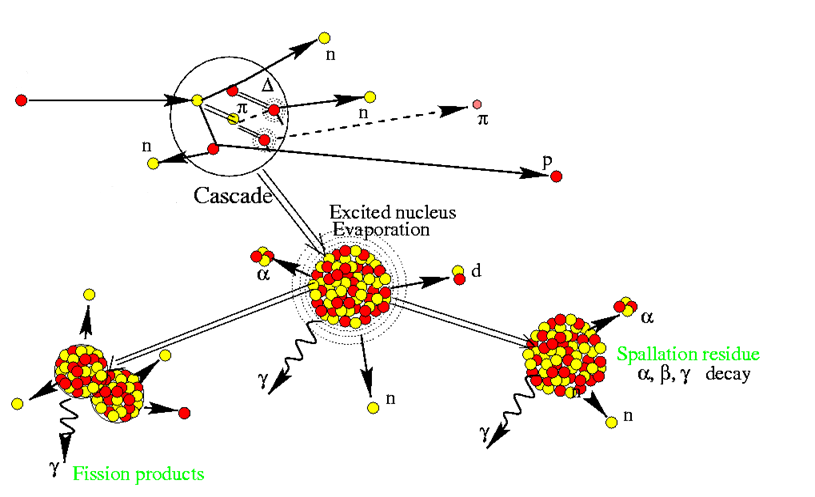
\includegraphics[width=0.8\textwidth]{images/inclScematic.png}  
\caption{\label{fig:inclschematic} Schematic diagram of cascade and evaporation models. Image courtesy of E.Haettner~\cite{ehaettner}.}
 
 \end{center}
 \end{figure}

\subsubsection{Binary cascade}
The binary cascade is a hybrid cascade model with certain aspects of a quantum mechanical dynamics model. The model is characterized as being based on binary scattering between reaction participants and nucleons within the nucleus.

In this model the nucleons are described as gaussian wave packages, a nucleus is then built up by combinations of these wave-packages:


\begin{equation}
\Phi(x,q_i,p_i,t) = \frac{2}{(L\pi)^{\frac{3}{4}}}\exp{(\frac{-2}{L(x - q(t))})^2+ip_i(t)x}.
\label{wavePackage}
\end{equation}


The Slater determinant is ignored. The 3-dimensional nucleus model in the binary cascade assumes a isotropic spherical nucleus. The nucleus density is described by a Woods-Saxon potential for heavy Ions, while lighter ions are described through a harmonic oscillator nuclear shell model. Almost all ions involved in the simulation in this paper are considered light by this definition. The nuclear density distributions are defined as 

\begin{equation}
\rho(r) = 
\begin{cases}
\begin{cases}
(\pi R^2)^{\frac{3}{2}}\exp{\frac{-r^2}{R^2}} & \text{A} \le 16 \text{  (Harmonic oscillator)}\\
\frac{\rho_{0}(R)}{1+\exp({\frac{r-R}{a}})} & \text{A} > 16 \text{  (Woods-saxon)}
\end{cases} & r \le R \\
0 & r > R. \\
\end{cases}
\label{binaryCascadePotential}
\end{equation}

Firstly, the participating nuclei are generated. The positions of the nucleons are randomly picked from these probability distributions. The Fermi-momentum for every nucleon is decided according to the Thomas-Fermi approximation $$p^{max}_F(r) = \hbar c [3 \pi^2 \rho(r)]^\frac{1}{3}.$$Secondly, $A-1$ nucleons are given a momentum between zero and the Fermi momentum. The last momentum is chosen so that all momentums even out. This is done by picking the negative sum of all other momentums. If the absolute value of the momentum happens to be above the Fermi momentum other momentums are repicked randomly until a satisfactory configuration is available.

The Binary cascade transportation algorithm starts by picking randomly the impact parameter from the disc that is perpendicular to the distance vector inbetween the center of the disc and the middle of the nucleus. The closest distance $d^{min}_{i}$ defined by straight-line trajectories are calculated for each nucleon in the nucleus. The binary cascade then proceeds to calculate the interaction cross-sections $\sigma_i$ with all target nucleons based on the momenta of the nucleon in the nucleus, and the projectile momentum. Nucleons that have a smaller interaction radius than their distance $d^{min}_{i}$ are considered as plausible interaction targets. These targets are listed according to their individual time-of-flight by straight-line trajectory $t^{tof}_i$. The primary particle is then transported in the nuclear field with steplengths of the magnitude of the difference between the different times of flight $$t_{step} = t^{tof}_i - t^{tof}_{i+1}$$The equations of motion are solved in the nuclear field by means of Runge-Kutta integration. If no collision is found a new nucleus and impact parameter is picked.
%fixme, below could be better formulated
Nucleon-nucleon interactions are based on experimental data and phenomenology. After collisions secondaries of the collision that are Pauli allowed, and above the Fermi momentum $p_F$, are traversed as new primaries. The Binary cascade does however not consider collisions inbetween participants.
%humm, why do we care about this if they are below fermi mometum anyway? or do we mean the different primaries?

The Binary cascade model proceeds as long as there are still particles above the kinetic energy threshold  of 75~MeV, or until the mean kinetic energy of the participants has dropped below 15~MeV. Once this phase is reached the nucleus is handed to the evaporation model.

\subsubsection{Geant4 evaporation model}

Once the cascade model has reached one of its cut-off criteria the remaining excited nucleus is passed on to the evaporation model which is a more statistical model based originally on the work of Weisskopf~\cite{Weisskopf}. In this model the nucleus is assumed to be in an equilibrium state.

The evaporation model takes the nucleus' excitation energy and isotope as input. On the basis of this data a statistical distribution is defined for the realized Monte Carlo events.

\subsubsection{Fission model}

The Geant4 fission model used in this work utilizes the empirically found relation for the distribution of fragments. Fission processes for a nucleon with atomic number $A_f$ have both symmetric and antisymmetric components, defining the total fission output as
\begin{equation}
 F(A_f) = F_{sym}(A_f) + \omega(U,A,Z) F_{asymm}(A_f).
\label{fissionSymmetricAsymmetric}
\end{equation}
Where $\omega$ defines the relative contribution of each component and is a function of the excitation energy U, and the atomic numbers of the fissioning nucleus.

From experimental data it has been found that good approximations for the functions $F_{sym}$ and $F_{asym}$ can be acquired with exponential fits on $A$ and $A_f$ as variables.

At given mass of fragment $A_f$ the experimental data on the charge $Z_f$ was found to be well described by a Gaussian fit. The average kinetic energy is described through the empirical relation $$<T_{kin}>=0.1178Z^2/A^\frac{1}{3} + 5.8$$. However, the kinetic energy distribution of the asymmetrically scattered fission products is known to have a greater mean than that of the symmetrically distributed ones, which also is compensated.

For further discussion of the Geant4 fission model the reader can consult the Geant4 physics reference manual~\cite[Chapter 31]{physicsManual}.

\subsubsection{Fermi break-up}

For light nuclei the excitation energy is often of the magnitude of the nucleon binding energy. Therefore it is possible to construct rather simple predictive statistical models for break-up. This approach was first introduced by Enrico Fermi and is thus called the Fermi break-up model. This model requires a nuclei with three times larger excitation energy than binding energy. Furthermore, $A < 12$ and $3(A - Z) < Z < 6$ is required. Fermi break-up can be seen as an extreme case of fissioning in the nucleus where the nucleus completely ``explodes``. %fixme: phase space should be mentioned
\clearpage
\section{Simulation setup} %practical aspects of simulation
The simulation is performed with the latest version of the Geant4 suite version 4.9.3b with the newest simulation models available in the distribution.

The simulation code is based around the hadrontherapy simulation produced by G.A.P. Cirrone, F. Di Rosa, S. Guatelli and  G. Russo of INFN Genova and Catania. This IAEA benchmark simulation is be distributed alongside the hadrontherapy example. This required varoius major changes in the code, including:
\begin{itemize}
\item The geometry, beam and beamline had to be rewritten to correspond to the experimental setup at GSI~\cite{ehaettner}, but in such a way that the geometries may be interchanged through macro commands. Rewriting the geometry also meant having to rewrite the detection code, which defines what is recorded and where.
\item Analysis was to be done in ROOT bypassing AIDA that is used by the hadrontherapy example.
\item One macro had to be able to perform multiple runs with different parameters.
\item Means of documenting the code through doxygen were implemented.
\end{itemize}


\begin{figure}[h] 
\begin{center}
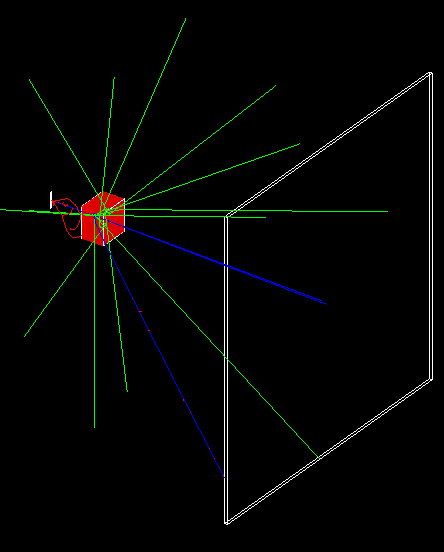
\includegraphics[width=0.5\textwidth]{images/oneEvent.png}  
\caption{\label{fig:oneEvent} One event with 27.9~cm thick water phantom.}
\end{center}
\end{figure}

\begin{figure}[h] 
\begin{center}
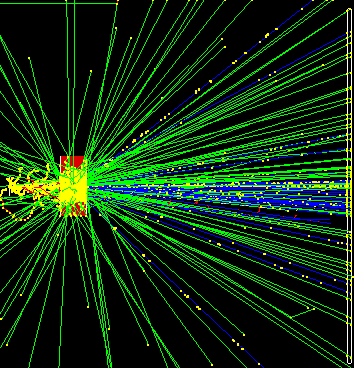
\includegraphics[width=0.5\textwidth]{images/twentyEvents.png}  
\caption{\label{fig:twentyEvents} Profile view of the simulation with the tracks recorded from 23 incident events with a 27.9~cm phantom. This clearly visualizes the yield of fragments has a clear forward directed distribution.}
\end{center}
\end{figure}

Reference data for the measurements involved in this paper have been acquired from GSI and were measured by E. Haettner in 2006 as part of her Master's thesis~\cite{ehaettner}. Haettner used two different setups for the measurements; measurements made with the H1 scintillation detector and attenuation measurements made at a shorter distance for calculating the Bragg-curve. In the following parts of this paper recreating these measurements through simulation is discussed. Firstly the required geometries are discussed, and secondly the used methods of picking and analyzing events are presented.

\subsection{Geometries}

\subsubsection{H1 measurements}

\ref{fig:haettnersetup3} shows the geometry Haettner used in angular and energy distribution measurements with the H1 detector. This ''H1 measurements`` setup was recreated in the simulation environment. The major differences being:
\begin{itemize}
\item The pipe in the water phantom was by inspection of photograph~\ref{fig:haettnersetup2} deemed impossible to recreate in such a way that it could be assumed to recreate any backscattering effects or similar induced by the pipe. Thus a simple cube-shaped phantom was used.
\item The water phantom had the cross-section of 50x60~cm. However, the beam exit-window had only an area of 32x8~cm. It was assumed that the detector was during angular experiments moved in the horizontal plane (the broader side of the window) and thus it was deemed a fair assumption to use a water phantom with a cross-section of 32x32~cm in the y-z plane. 
\item The detector itself was a large scoring plane registering all incoming particles. The measurements were analyzed in ROOT. This allowed to minimize the amount of time-consuming simulation-runs by assuming symmetry.
\end{itemize}

Through personal correspondence with E.Haettner it was confirmed that the indicated water-thicknesses in the data are the actual phantom thicknesses augmented by the water-equivalents of the other parts of the experiment. Data recorded through the simulation should be compared to the actual water-thicknesses because the effects of these other elements are simulated as well. During the July H1 measurements the water-equivalents were approximated to be 8mm. Thus, the water-thickness to be used in the simulation of a experimental datapoint is that depth subtracted by 8mm. %should be noted unknown constant in haettner's data of small magnitude. Also in February there was apparently more WE, but how much?

\subsubsection{Bragg-curve measurements}
In this paper the Bragg-curve is calculated by imaginary voxel-layers in the phantom, and therefore is only of interest in compensating the water equivalents added by Haettner into the results for the different parts of the experiment.

This means that data acquired through the simulation technique used should be compared to values with the water-equivalents subtracted. Haettner's GSI experimental setup for the Bragg-curve had an WE of 0.578~cm according to~\cite[table 4.1]{ehaettner}.


\begin{figure}[!ht]
\centering
\subfigure[]{
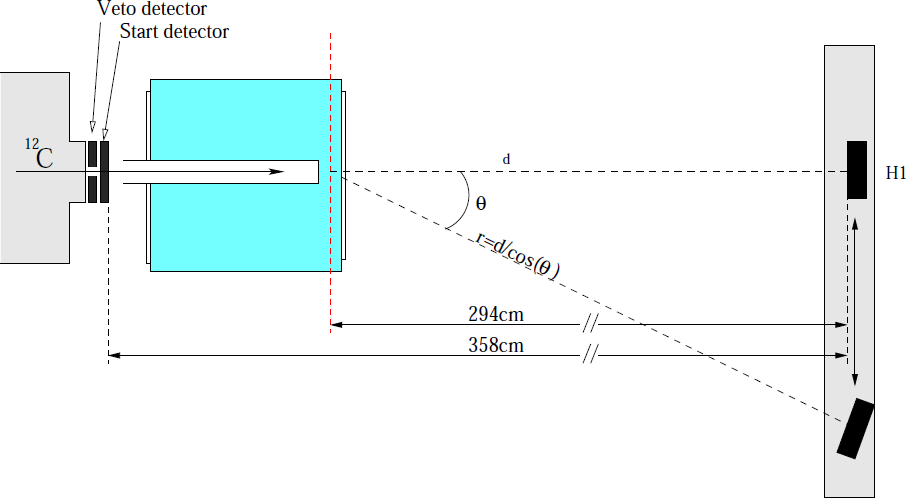
\includegraphics[width=0.9\textwidth]{images/haettnersetup3.png}
\label{fig:haettnersetup3}
}
\subfigure[]{
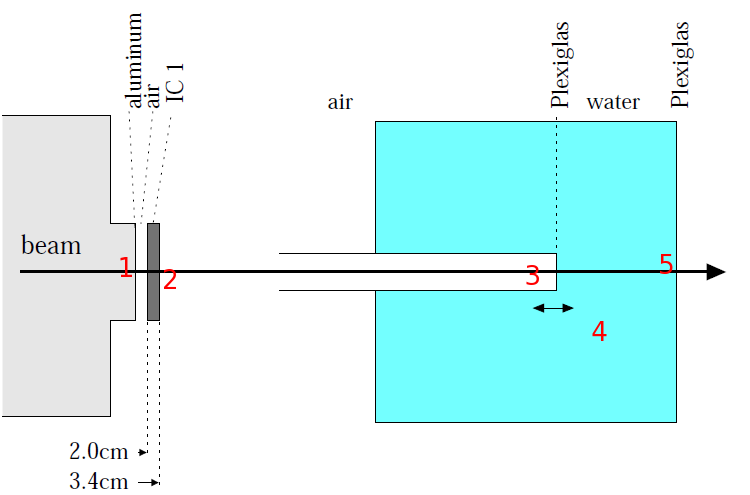
\includegraphics[width=0.9\textwidth]{images/haetnnersetup2.png}
\label{fig:haettnersetup2}
}
\label{fig:EHaettnerDataForAEDistrib1}
\subtable[]{
\begin{tabular}{llll} %fixme: this should be more of a caption
& & \textbf{Material} & \textbf{Thickness} \\
1&Beam source window &Aluminum&0.1~mm\\
2&Ionization Chamber 1 &Air-equivalent&1.4~cm\\
3&Adjustable tube window &Plexiglas&2~mm\\
4&Phantom &Water& 0-40~cm\\
5&Container back-window &Plexiglas&2~mm\\
\end{tabular} 
}
\caption[Optional caption for list of figures]{(a) experimental setup for measurements made with the H1 detector. In this paper and the simulation-code the angle denoted by Haettner with $\theta$ is denoted $\phi$. (b) Geometry and elements in water phantom. (c) Materials and thicknesses along beam path. Images courtesy of E.Haettner~\cite{ehaettner}.}
\label{fig:ShouldGiveTableAndFigure}
\end{figure}

\begin{figure}[h] 
\begin{center}
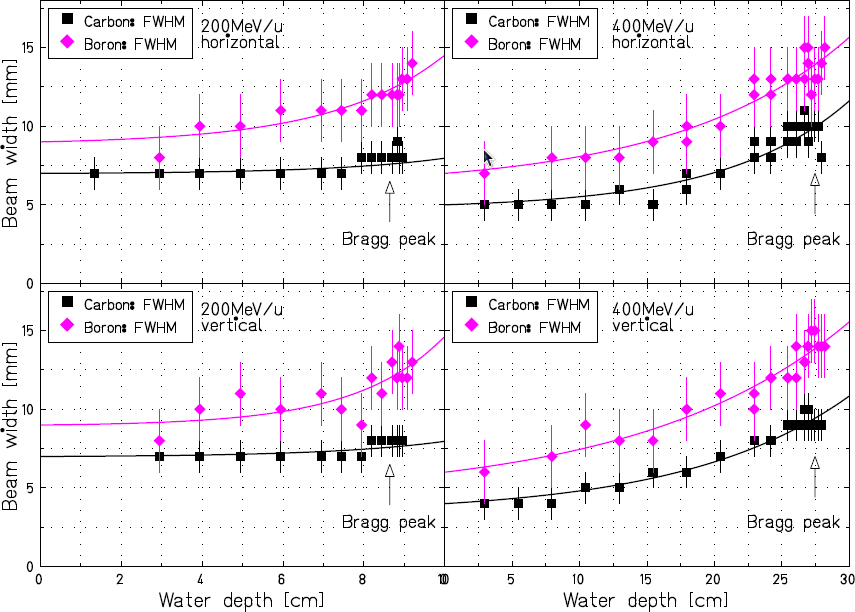
\includegraphics[width=0.9\textwidth]{images/haettner48.png}  
\caption{\label{fig:haettner48} Experimental measurements of the relation between the depth in water and FWHM of the incident Carbon beam and fragmented Boron. Figure courtesy of E.Haettner.~\cite{ehaettner}}
 \end{center}
 \end{figure}

\subsection{Characterizing Carbon beam shape for simulation}

%0.2^2/(3+0.279/2)^2

The beam is considered a pen-shaped beam. Haettner has performed measurements to define the beam's characteristics.

Firstly, Haettner evaluates the accuracy of the beam's energy to be $\Delta E/E\approx5\times10^{-3}$, meaning that the energy distribution of the beam is very narrow. This error was simulated with a gaussian distribution with the standard deviation 1~MeV/u and 2~MeV/u for the 200 respectively 400~MeV Beams.

Secondly, Haettner further characterizes the beam by measuring it in air at three distances (0~m,1~m and 3~m). The incident beam was assumed to be parallel before leaving the vacuum tube window, thus assuming recorded enlargement of the beam's FWHM is explainable simply by the scattering from the exit-window and air. However, in this paper these results could not be verified and thus a very small deviation in the beam's angular distribution was introduced (chapter ~\ref{beamShapeAnalysis}). The initial width of the beam was assumed normally distributed and thus the original 4~mm FWHM of the beam width was reproduced by picking beam $y$ and $z$ deviations from a normal distribution with $\sigma = 1.7$~mm according to the relation $$\mathrm{FWHM} =   2 \sqrt{2 \ln 2 } \; \sigma \approx 2.35482 \; \sigma$$

In experimental work~\cite{ehaettner} proceeds to analyze the scattering of the beam with variable water thicknesses, shown in figure ~\ref{fig:haettner48}. However, even though the overall distribution produced in our results(Appendix~\ref{AppendixA}) was in line with experimental data the FWHM measure was not good for comparison due to the missing height of the forward peak.

%\subsection{Water tank}
%The water phantom had in the experiment the cross-section of 50x60cm. However, the beam exit-window had %only an area of 32x8 cm, and the physical parameters of what covered other parts was unknown. Therefore it %was assumed that the detector was during angular experiments moved in the horizontal plane (the broader %side of the window) and thus it was deemed a fair assumption to use a water phantom with a cross-section of %32x32cm in the y-z plane. This regrettably makes it impossible to study backscattering and similar effects %with high precision.

\subsection{Definition of read-out geometry}

\subsubsection{Beam attenuation}

In order to calculate the Bragg curve of the beam a water phantom of 40~cm was placed in the path of the beam. The amount of water was approximated on the basis of GSI data so that the entire Bragg-curve and a considerable part of the fragment-tail would be visible. This water phantom was divided into 400x1x1 primitive scorer voxels. This in effect means the water phantom was presented as 400 water-slices placed perpendicular to the beam. The Bragg-peak is calculated by saving the energy-deposits in every slice. Thus a histogram of a characteristic Bragg-curve is recorded.

\subsubsection{Definition of angular values\label{AngularDistributionText}}

\begin{figure}[!h] 
\begin{center}
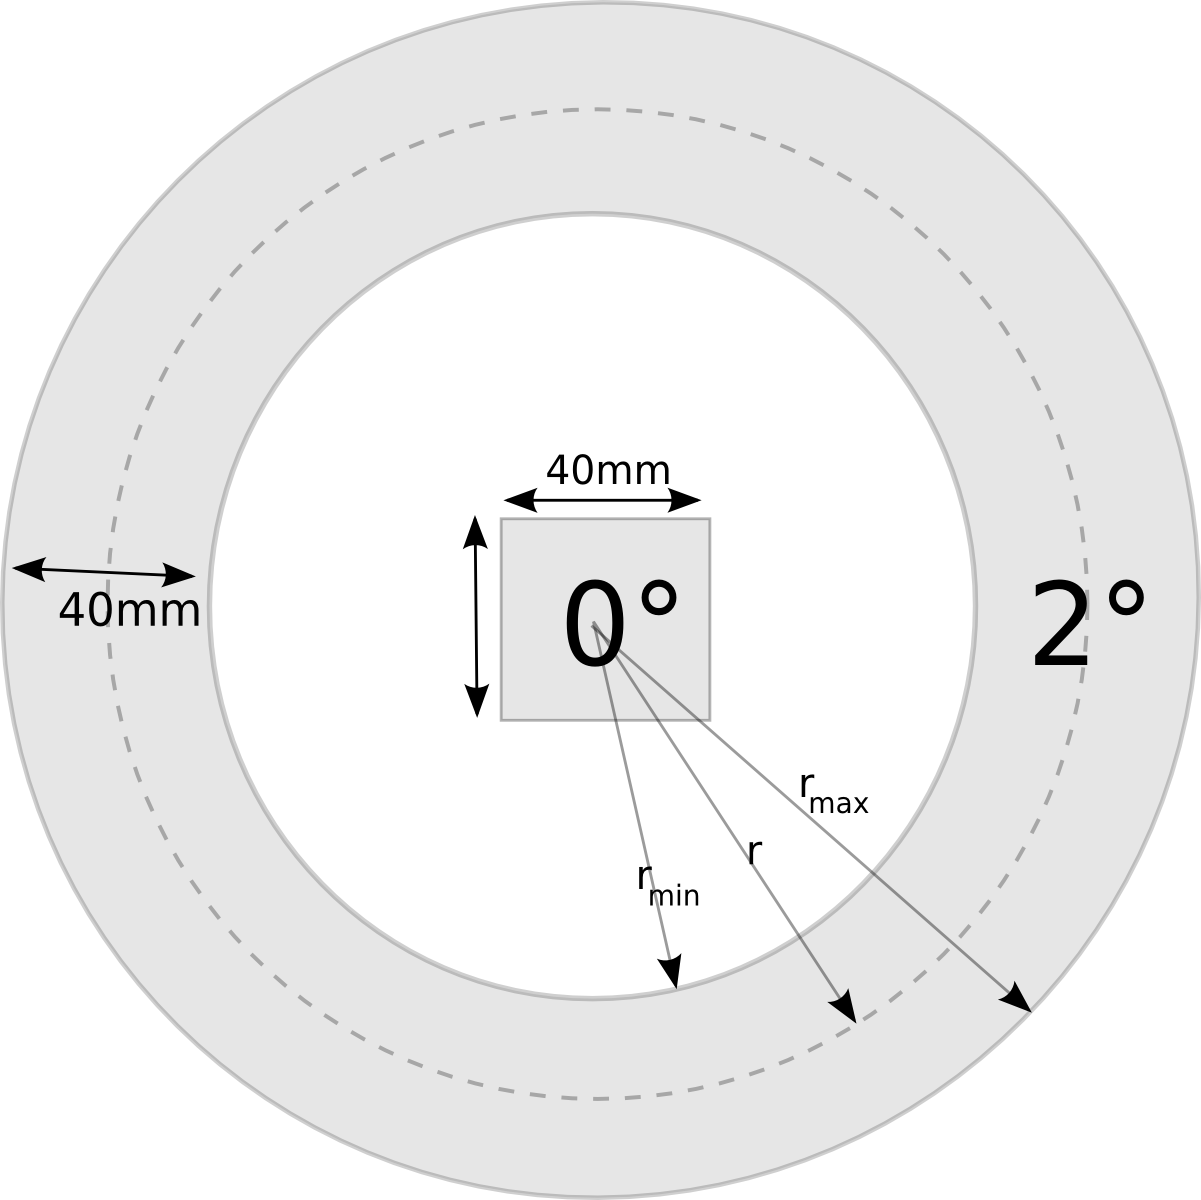
\includegraphics[width=0.6\textwidth]{images/annulus.png}  
\caption{\label{fig:annulusesExplained} Schematic picture of read-out area for charged fragments. The zero degree angle is read out from a square detector while larger than zero degree angles are read out with consecutive circle annuluses where $r$ is seen at the given angle from the middle of the water phantom. The annulus width a is determined trigonometrically for each angle of analysis in order to correspond to the solid angle covered by H1.}
\end{center}
\end{figure}

A detector distance of 298.5~cm is used as described in fig \ref{fig:haettnersetup3}. In the original experiment the H1 detector was moved and yields at different angles were recorded and plotted as a function of the angle at which the detector was seen. However, in order to increase effectiveness of the simulation circle annuluses were used as read-out areas at angles greater than zero. For the events recorded at 0 degree angle a square detection area was used. This approach is a slight approximation when it comes to small non-zero angles as the flux of the detection area may not be considered exactly similar to that of a square detector at that angle.

The annulus width $a$ was determined so that it covered all of the solid angle that the tilted detector would cover while rotated around the beam axis. Thus the width of the annulus a is a function of $\phi$ according to the relation $$a(\phi) = \text{H1 sidelength} \times [\cos(\phi)+ \cot(\frac{\pi}{2} - \phi - \Delta\phi)\sin(\phi)],$$where $$\Delta\phi = \arctan(\frac{2 \times \text{scattering distance}}{\cos(\phi) \times \text{H1 sidelength}})$$ is the angle subtended by $r$ to $r_{min}$ and $r_{max}$ respectively.
%fixme, that's got to be possible to simplify a bit.
Results were divided by the amount of events and normalized to the solid angle of the detection area.

The volume a square detector pointed towards the source at distance $s$ solid angle fills up is a pyramid. Thus, the formula $\Omega_{square} = 4 \arcsin(\frac{\text{(H1 sidelength)}^2}{4d^2+\text{(H1 sidelength)}^2})$ for the solid angle of a pyramid describes the solid angle subtended by the detector H1 at distance $d = \frac{\text{scattering distance}}{\cos(\phi)}$ from the middle of the water phantom.

The circle annuluses used as read-out areas subtend the solid angles $$\Omega_{annulus} = 2 \pi [\cos(\phi - \Delta\phi) - \cos(\phi + \Delta\phi)]$$. When $\phi \le \Delta\phi$ the read-out area reduces to a circle with the solid angle $$\Omega_{circle} = 2 \pi [1 - \cos(\phi + \Delta\phi)]$$.

%\begin{comment}
%Koska lupasin koordinoida speksien määärittelyn.
%voisit Gillis tehdä raporttiisi seuraavaksi alaluvun :
%'Characterization of the primary beam and experimental setup for the
%IAEA benchmark'
%Ennen kun rupeat rakentamaan Geant4 simulaatiota  voisit siis kerätä
%Emman työstä
%kaikki vaadittavat tiedot (etäisyydet, materiaalit, dimensiot, beamin
%tiedot) tähän lukuun.
%Tämän tekstin tulisi olla itsenäinen osa opinnäytetyötä jotta sen voi
%kätevästi jakaa muiden Monte-Carlo koodien edustajlle.
%(Näppärä taulukko ja kuva kuten gradussa selventävät asiaa.) Tekstin
%pohjalta pitää pystyä luomaan
%yksikäsitteisesti oikeanlainen Monte-Carlo koe jonka tuloksia sitten
%verrataan Emman mittauksiin.

%doc/talk/images/inclSummary.png
%images/haettnersetup.png
%\end{comment}

%\subsection{Analysis}
%The simulation setup generates relatively little data. Thus an approach with separate analysis was chosen. %All events hitting the detectors were recorded and suitable ones were chosen in the analysis software ROOT.
\begin{comment}
\subsection{Simulation parameters}
%tarvitaanko?
The following table gives an impression of the amount of events used for each
\begin{itemize}
 \item Fragment energydistribution: 500 000 events, cuts 0.4
 \item Angular distributions: one run per depth (5.9,15.9,27.9,31.2,31.4), 100 000 events.
 \item Beam shape, 10 000 events, reiterated until empirically the best fit was found
\end{itemize}
\end{comment}

\clearpage
\section{Comparison of simulation results to GSI data}

This work focused much on the fragments generated in the water phantom. Thus, much of the work has been put into analyzing the different distributions of these fragments as they leave the water phantom. In this section angular both angular and energy distributions will be presented for different water phantom thicknesses and they will be compared to data from E.Haettner. The thicknesses are chosen so that the distributions can be viewed for the beam both ahead and behind the Bragg peak.

\subsection{Simulated carbon beam shape vs. measurements\label{beamShapeAnalysis}}
\begin{center}
 \begin{table}[!h]
\begin{tabular}{cccc} %fixme:
\textbf{Distance} & \textbf{GSI measurement (H$\times$V)} & \textbf{Straight incident beam} & \textbf{Added scattering} \\
0~m &4x4~mm& 3.9~mm & 3.9~mm\\
1~m &5x4~mm & 4.2~mm & 4.8~mm\\
3~m &11x9~mm& 5.2~mm & 9.0~mm\\
\end{tabular} 
\caption{\label{fig:beamFWHMtable} The beam FWHM as measured in experiment and reproduced in simulation and modified simulation.}
\end{table}
\end{center}
The particle beam shape was set so that measured 0~cm distance scattering of 4mm FWHM was duplicated. When this scattering experiment was repeated for the two other provided measurement points of 1~m and 3~m results were not in line with those of experimental data. We assumed further scattering not accounted for in the beam must have taken place. To include the added scattering a gaussian shaped stochastical deviation was introduced in the beam's momentum vector. This error was symmetrical in $y$ and $z$ with the magnitude of $1\permil$ of the x-component. This error was empirically chosen. The results are summarized in table~\ref{fig:beamFWHMtable}.


\subsection{Fragment yields (0$^\circ$-10$^\circ$)}
The experimental data was provided with interpolated estimates for the yields inside a 10 degree angle. This estimate is based on numerically integrating the angular distribution through a fitted normal distribution on low angles and a exponential fit at the larger angles. This yielded relatively large error margins, especially for the larger fragments. Comparable results were produced by picking all events within a circle with the radius $r = \text{scattering distance} \times \tan(10^{\circ})$ around the zero degree position.

The results and comparison are gathered in appendix~\ref{AppendixB}. The agreement is rather good for most fragments, however a considerable deviations from experimental data is viewable for Helium.

\subsection{Energy distribution of fragments}
\begin{figure}[h] 
\begin{center}
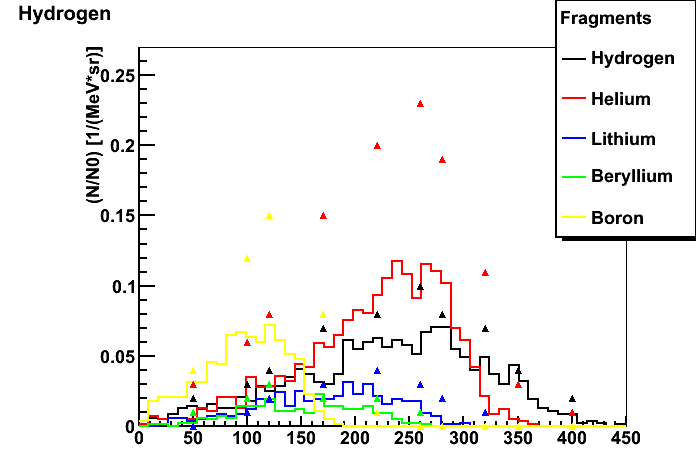
\includegraphics[width=0.9\textwidth]{images/fragmentEnergyDistr.png}  
\caption{\label{fig:fragmentEnergyDistr} Fragment energy distribution. Triangles are experimental data, solid lines Geant4 simulation. Water phantom thickness was 27.9~cm (slightly beyond the Bragg-peak)}
\end{center}
\end{figure}
The data was normalized for bin-width (9~MeV) and the solid angle of the square H1 detector centered at $0^{\circ}$ angle from the mean direction of the beam.

The shape of the results are mostly in line with the experimental data. However, the yield of Helium is clearly smaller than that of experimental results, also the peak for Boron is considerably lower than in experimental data. These phenomena are repeated also in other water-depths.

\subsection{Angular distribution of fragments}
\begin{figure}[!h] 
\begin{center}
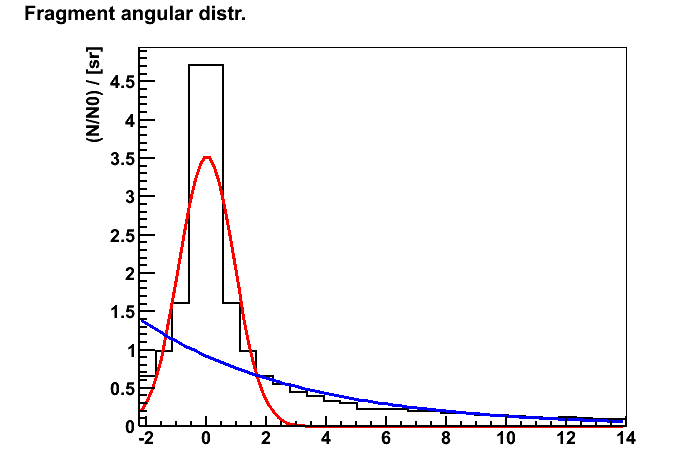
\includegraphics[width=0.7\textwidth]{images/plots/angularDistributions/equlBinnedHydrogen279.png}  
\caption{\label{fig:binnedHydrogen} Scattering angles for hydrogen binned at equal bin lengths. Gaussian and exponential fits are applied.}
 \end{center}
 \end{figure}
The angular distributions were simulated for a number of phantom-depths before and after the Bragg peak at about 27~cm. Results were normalized per number of incident ions and solid angle. The results were plotted against GSI data and in appendix~\ref{AppendixA}. The simulations were run with phantom thicknesses that were subtracted of water-equivalents. Through personal correspondence with E.Haettner it was apparent that the measurements made in July were compensated with a $0.8$~cm water equivalent for the non-water parts of the experiment

Results for $\phi \in [0,\arctan(\frac{\text{H1 sidelength}}{2 \times \text{scattering distance}}) \approx 0.4^{\circ}]$ were discarded in the plots due to the amount of stochastic error in this interval. These stochastic effects arose due to the annulus read-out area approximation when $r_{min} = 0$.

The obvious difference to the experimental data is the clearly lower yields at low angles. This relation is apparent for almost all depths and fragments that were analyzed. The difference seems to be accentuated for the lighter fragments. As beam attenuation data matches rather well the lack of forward yield may indicate that the simulation models scattering of fragments is too isotropic.

In figure~\ref{fig:binnedHydrogen} the angular distributions were recorded so that all detected hydrogen fragments were binned in a equal bin-width histogram according to scattering angle. This exemplifies well how the distribution is at small angles best described by a Gaussian shape while at larger angles an exponential function is a better fit. The need for a two-component model has been observed by several authors (Haettner~\cite{ehaettner}, Gunzert-Marx~\cite{gunzert-marx}, Golovkov~\cite{golovkov}). However as this approach differs from the one used by E. Haettner this graph is not comparable to her results. The results in the appendices mimic that approach by having variable size bins.

All in all the results seem in comparison to the experimental data fair for a hadronic Monte Carlo model.

\subsection{Angular energy distribution of fragments}
The angular energy plots were normalized for solid angle, number of events and bin-width. Although also here it is obvious the yields are too small at small angles, the shape of the distribution seems a satisfactory match. Similar indications were obtained with other fragments and depths as well. However, this graph verifies the missing forward-yields energy is equally distributed to the rest of the detected fragments.

Data for the energy distributions can here only be compared to a copy directly from the publication due to data-files for this distribution not being available to the author at the time of writing.

\begin{figure}[!ht]
\centering
\subfigure[Experimental data]{
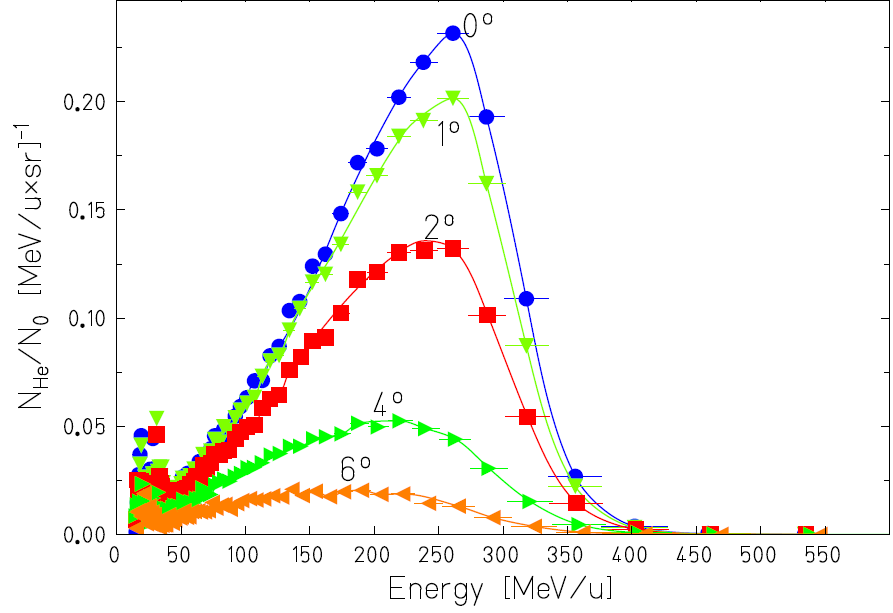
\includegraphics[width=0.45\textwidth]{images/plots/angularEnergyDistributions/EHaettnerDataForAEDistrib1.png}
\label{fig:EHaettnerDataForAEDistrib1}
}
\subfigure[Simulation data]{
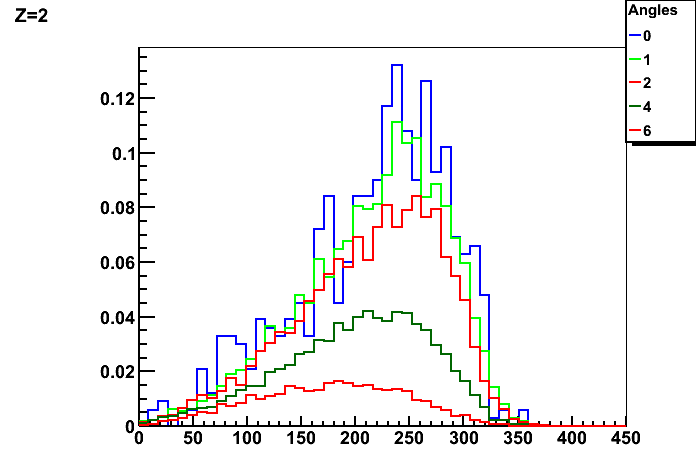
\includegraphics[width=0.45\textwidth]{images/plots/angularEnergyDistributions/AEDistrib2.png}
\label{fig:AEDistrib1}
}
\label{fig:AngularEnergyDistribution}
\caption[Optional caption for list of figures]{The angular energy distributions with a 27.9~cm water phantom. Although the yields at small angles seems to be clearly smaller in simulations than in experiments the distribution of energies is a fair match.}
\end{figure}

\subsection{Bragg curve}
The Bragg peak was measured from the simulation data to be located at $27.16 \pm 0.05$~cm which is a rather good match with the experimental result of 27.46~cm. This difference alone was not deemed as sufficient to explain the missing forward-yield.

The greatest difference is the average ionization per meter in water, which is about 50 percent larger in the experimental data. %fixme, is this really so

%should the fluka analysis be mentioned?

\begin{figure}[h] 
\begin{center}
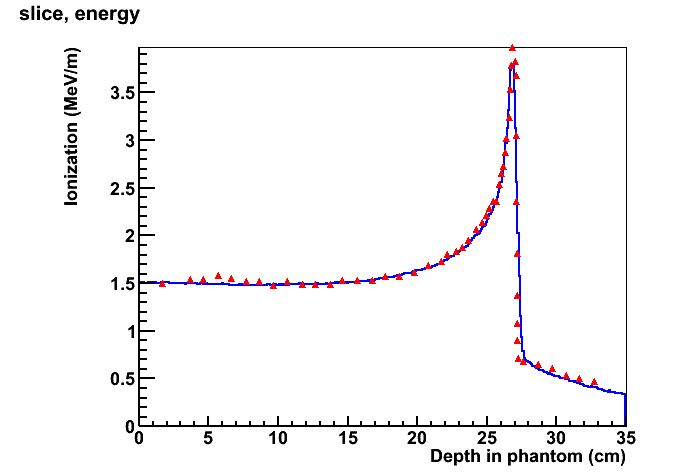
\includegraphics[width=0.9\textwidth]{images/plots/braggPeak/braggPeakComparisonToData.png}  
\caption{\label{fig:braggPeakCompared} Normalized Bragg Curve, experimental data is red and Geant4 simulation blue.}
 \end{center}
 \end{figure}

\clearpage
\section{Conclusion and outlook}
Considering the relative quality of prediction of Monte Carlo models for hadronic physics it may be concluded that results all in all were pretty well in line with the experimental data. However, it is clear that there are certain discrepancies are viewable in the results which are not within the error-margins of the experimental work.

Further work is needed to determine the cause of these lacks in yields. As a good starting hypothesis one may choose to research the isotropicity of the evaporation model, because the missing yields at low angles is especially apparent for light fragments.

For this work the detection-voxels in the phantom need to be changed to the \textit{G4SensitiveDetector} type from \textit{G4PrimitiveDetector}. This change will allow better analysis of what happens inside the water phantom instead of just the analysis of the resulting fragments that was focused on in this paper.

The experimental data pool of carbon beams is rather limited, and the paper by E.Haettner used as reference in this article is one of the more thorough ones with relatively good possibilities for recreating the experiment and compare the data. However, there remains a number of things in this experiment that were not recreatable in the simulation code.

The author hopes by this paper to provide a contribution to the pool of carbon treatment related simulation analysises, and ease the development of models.

The author also studied others models for hadronic simulations. The original intent of this paper was to perform the simulations with INCL and ABLA code. However, the anticipated release of the INCL code supporting light-nucleus interactions has not been released at the time of writing. This work is therefore left for the future, with a good adaptable GEANT4b framework and related ROOT analysis scripts. The theoretical bases of the INCL and ABLA codes are introduced in this paper in appendix~\ref{appendixincltheory}.

\clearpage

\bibliographystyle{unsrt} \bibliography{refs.bib} 

%%%%% Liitteet 
\appendix 

\clearpage
\addcontentsline{toc}{section}{Appendices}
\section{\label{AppendixA}: Angular Distributions of charged fragments.\label{AngularDistributionAppendix}}

The following graphs present the angular distributions of the scattered fragments. Data is collected for five different depths both ahead and beyond the Bragg-peak separately for all fragments. Red triangles represent data from E. Haettner~\cite{ehaettner}, blue crosses the Monte Carlo simulation described in chapter~\ref{AngularDistributionText}.

%% Liitteiden kaavat, taulukot ja kuvat numeroidaan omana kokonaisuutenaan
\renewcommand{\theequation}{A\arabic{equation}}
\setcounter{equation}{0}  
\renewcommand{\thefigure}{A\arabic{figure}}
\setcounter{figure}{0}
\renewcommand{\thetable}{A\arabic{table}}
\setcounter{table}{0}
\renewcommand\thesection{A}
\setcounter{section}{1}

\subsection{Hydrogen}
\begin{figure}[!h]
\centering
\subfigure[5.1~cm, Bad correlation. However, experimental data has large uncertainty due to carbon interference.]{
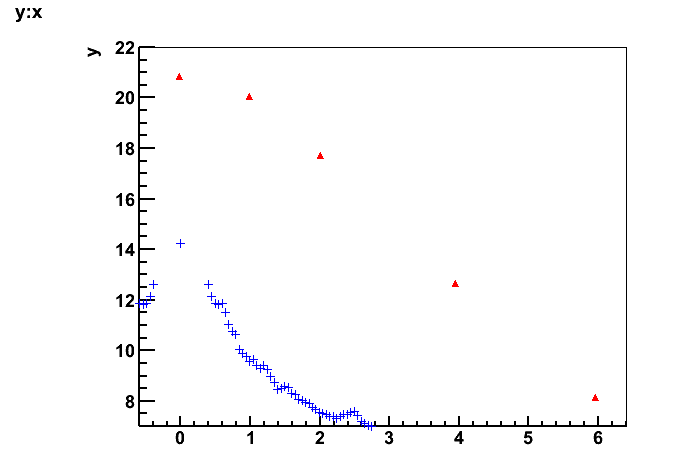
\includegraphics[width=0.43\textwidth]{images/plots/angularDistributions/AD_59_1_N.png}
\label{fig:AD_5.9_1_N}
}
\subfigure[15.1~cm]{
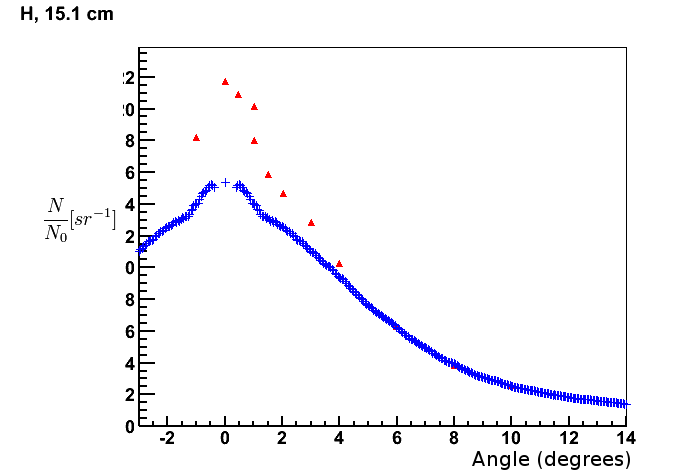
\includegraphics[width=0.43\textwidth]{images/plots/angularDistributions/AD_159_1_N.png}
\label{fig:AD_15.9_1_N}
}
\subfigure[27.1~cm]{
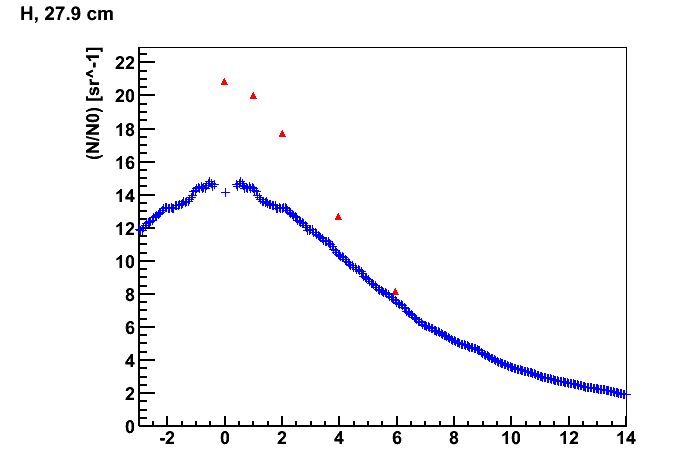
\includegraphics[width=0.43\textwidth]{images/plots/angularDistributions/AD_279_1_N.png}
\label{fig:AD_27.9_1_N}
}
\subfigure[30.4~cm]{
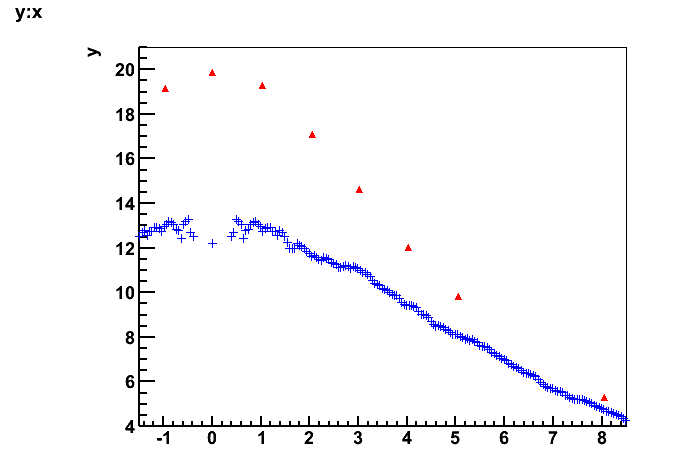
\includegraphics[width=0.43\textwidth]{images/plots/angularDistributions/AD_312_1_N.png}
\label{fig:D_31.2_1_N}
}
\subfigure[33.9~cm]{
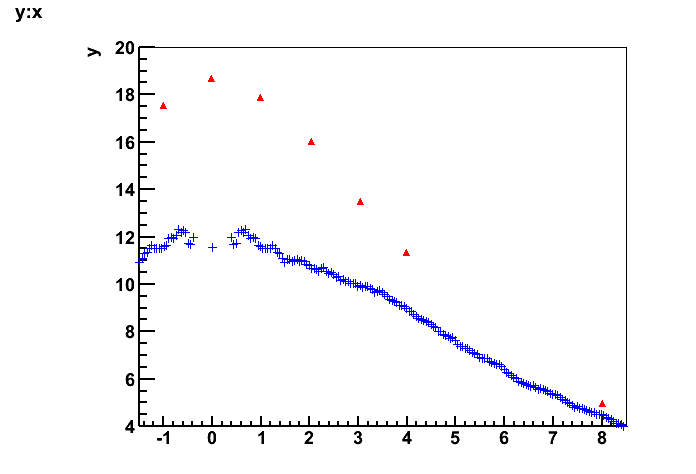
\includegraphics[width=0.43\textwidth]{images/plots/angularDistributions/AD_347_1_N.png}
\label{fig:D_34.7_1_N}
}
\label{fig:subfigureExample}
\caption[Optional caption for list of figures]{Angular distribution of hydrogen fragments.}
\end{figure}
\clearpage
\subsection{Helium}
\begin{figure}[!ht]
\centering
\subfigure[5.1cm]{
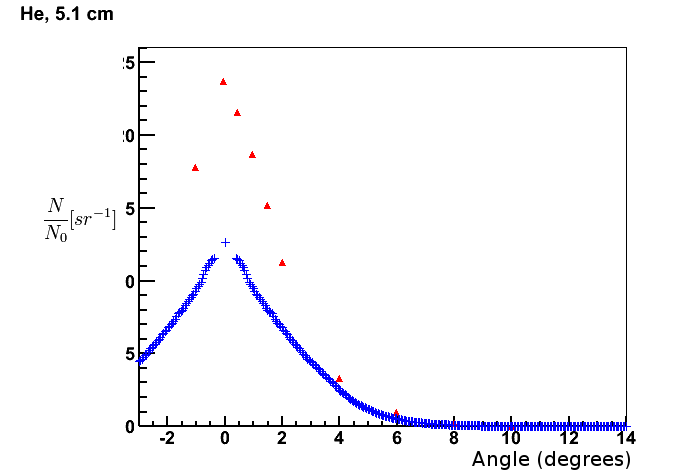
\includegraphics[width=0.45\textwidth]{images/plots/angularDistributions/AD_59_2_N.png}
\label{fig:AD_5.9_2_N}
}
\subfigure[15.1cm]{
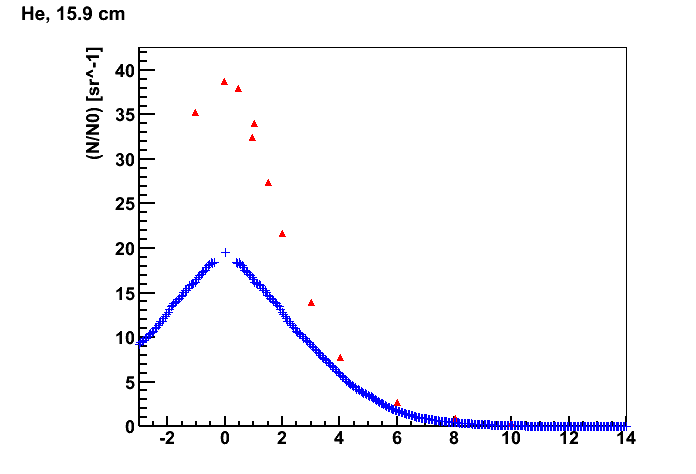
\includegraphics[width=0.45\textwidth]{images/plots/angularDistributions/AD_159_2_N.png}
\label{fig:AD_15.9_2_N}
}
\subfigure[27.1cm]{
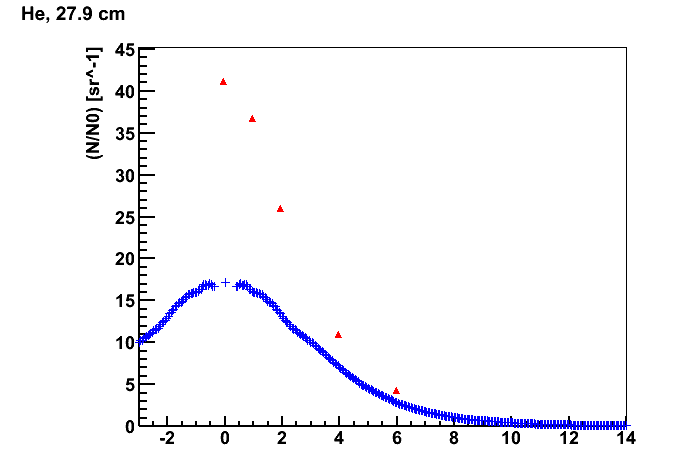
\includegraphics[width=0.45\textwidth]{images/plots/angularDistributions/AD_279_2_N.png}
\label{fig:AD_27.9_2_N}
}
\subfigure[30.4~cm]{
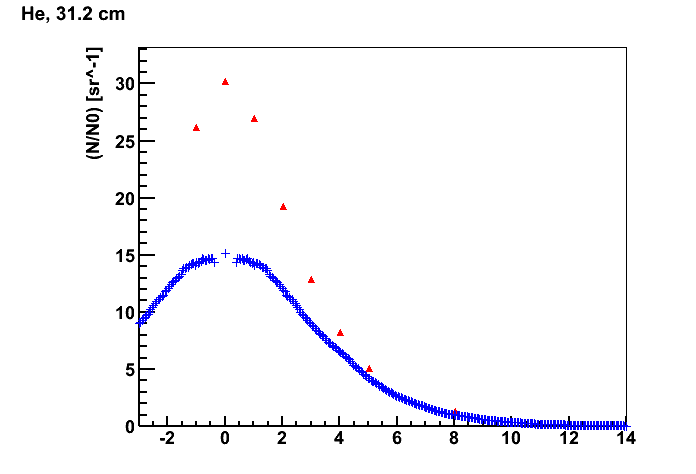
\includegraphics[width=0.45\textwidth]{images/plots/angularDistributions/AD_312_2_N.png}
\label{fig:D_31.2_2_N}
}
\subfigure[33.9~cm]{
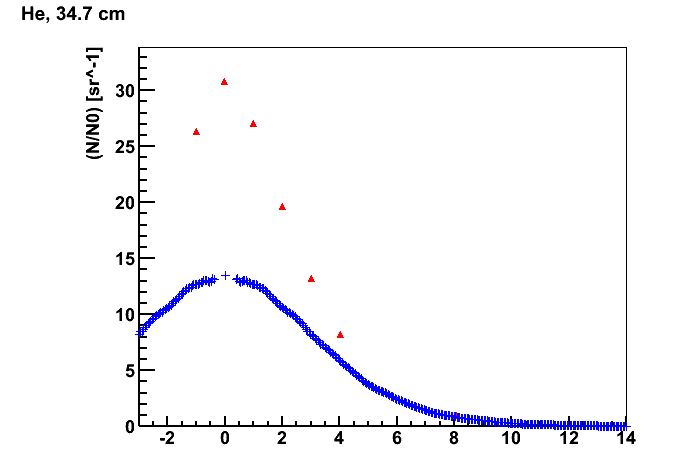
\includegraphics[width=0.45\textwidth]{images/plots/angularDistributions/AD_347_2_N.png}
\label{fig:D_34.7_2_N}
}
\label{fig:subfigureExample}
\caption[Optional caption for list of figures]{Angular distribution of helium fragments.}
\end{figure}
\clearpage
\subsection{Lithium}
\begin{figure}[!ht]
\centering
\subfigure[5.1cm]{
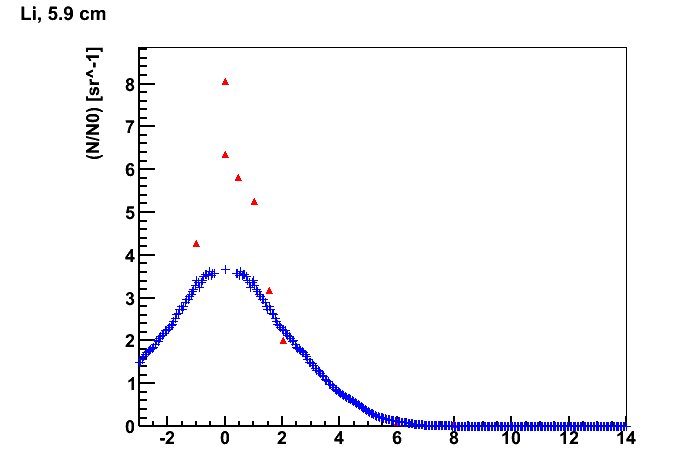
\includegraphics[width=0.45\textwidth]{images/plots/angularDistributions/AD_59_3_N.png}
\label{fig:AD_5.9_3_N}
}
\subfigure[15.1cm]{
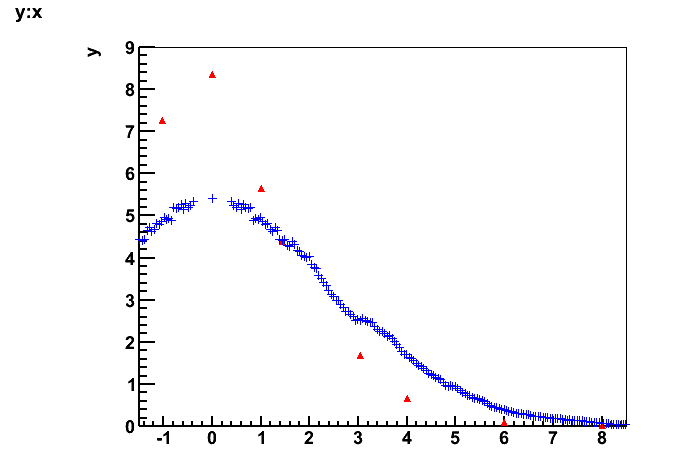
\includegraphics[width=0.45\textwidth]{images/plots/angularDistributions/AD_159_3_N.png}
\label{fig:AD_15.9_3_N}
}
\subfigure[27.1cm]{
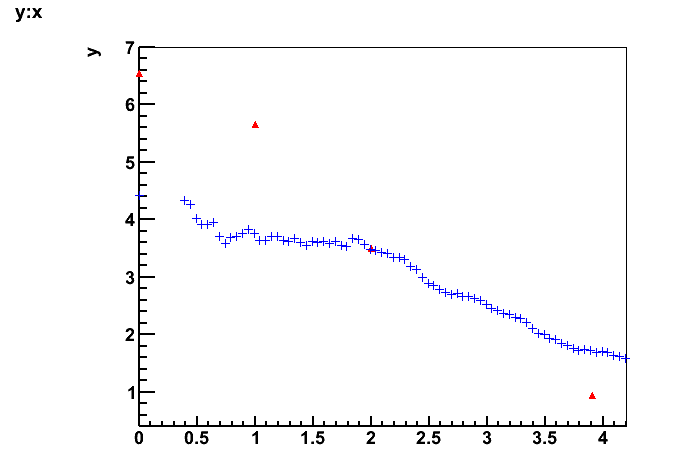
\includegraphics[width=0.45\textwidth]{images/plots/angularDistributions/AD_279_3_N.png}
\label{fig:AD_27.9_3_N}
}
\subfigure[30.4~cm]{
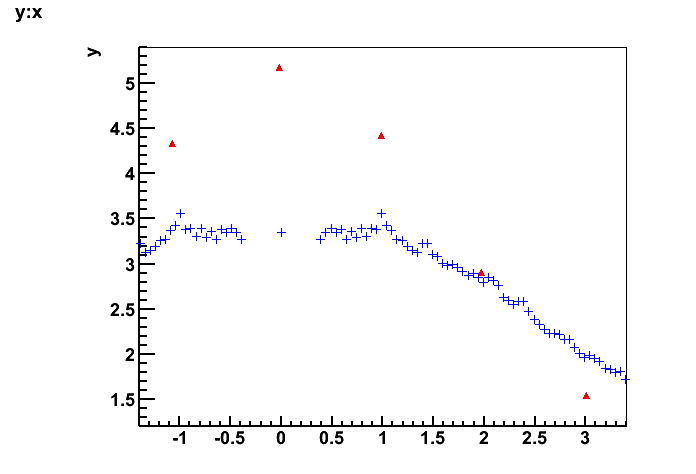
\includegraphics[width=0.45\textwidth]{images/plots/angularDistributions/AD_312_3_N.png}
\label{fig:D_31.2_3_N}
}
\subfigure[33.9~cm]{
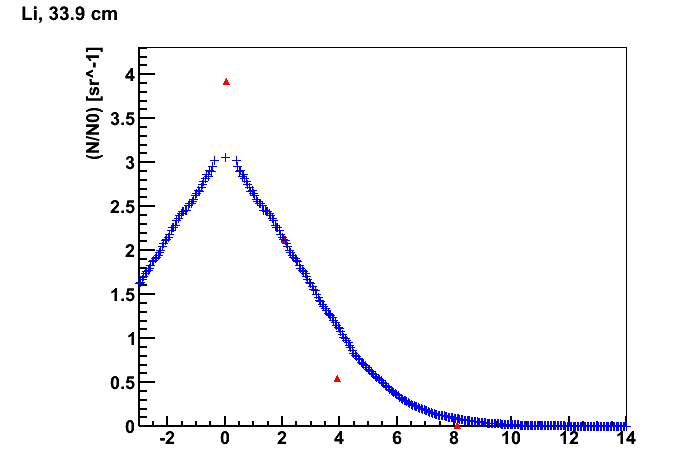
\includegraphics[width=0.45\textwidth]{images/plots/angularDistributions/AD_347_3_N.png}
\label{fig:D_34.7_3_N}
}
\label{fig:subfigureExample}
\caption[Optional caption for list of figures]{Angular distribution of lithium fragments. The double-peak in \subref{fig:D_31.2_3_N} is a statistical error due to small sample.}
\end{figure}
\clearpage
\subsection{Beryllium}
\begin{figure}[!ht]
\centering
\subfigure[5.1cm]{
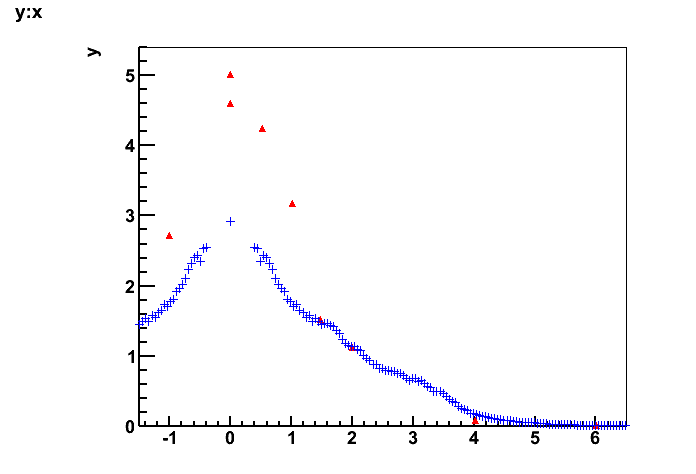
\includegraphics[width=0.45\textwidth]{images/plots/angularDistributions/AD_59_4_N.png}
\label{fig:AD_5.9_4_N}
}
\subfigure[15.1cm]{
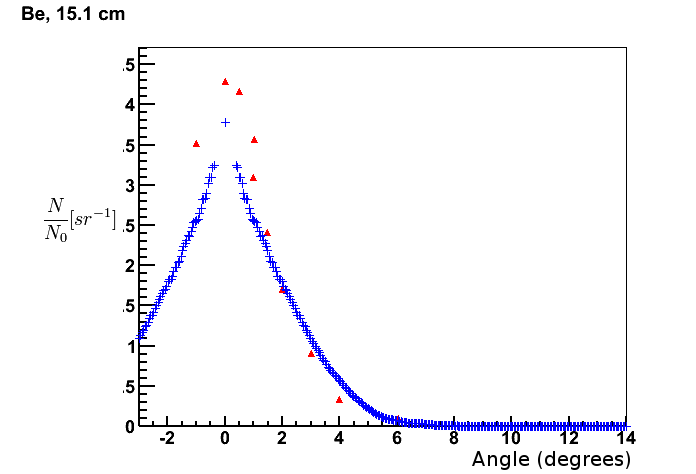
\includegraphics[width=0.45\textwidth]{images/plots/angularDistributions/AD_159_4_N.png}
\label{fig:AD_15.9_4_N}
}
\subfigure[27.1cm]{
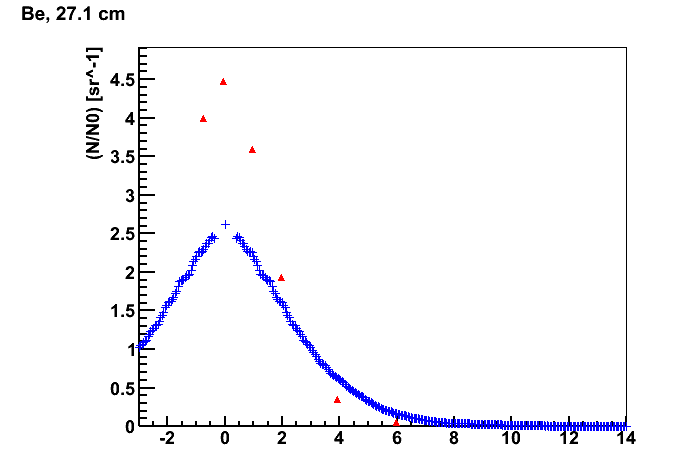
\includegraphics[width=0.45\textwidth]{images/plots/angularDistributions/AD_279_4_N.png}
\label{fig:AD_27.9_4_N}
}
\subfigure[30.4~cm]{
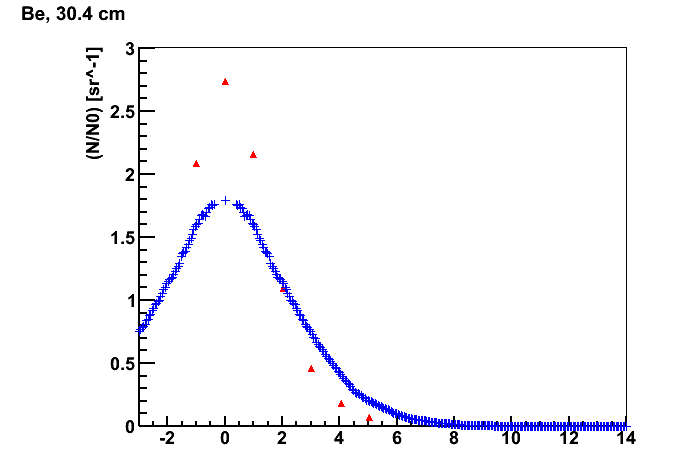
\includegraphics[width=0.45\textwidth]{images/plots/angularDistributions/AD_312_4_N.png}
\label{fig:D_41.2_4_N}
}
\subfigure[33.9~cm]{
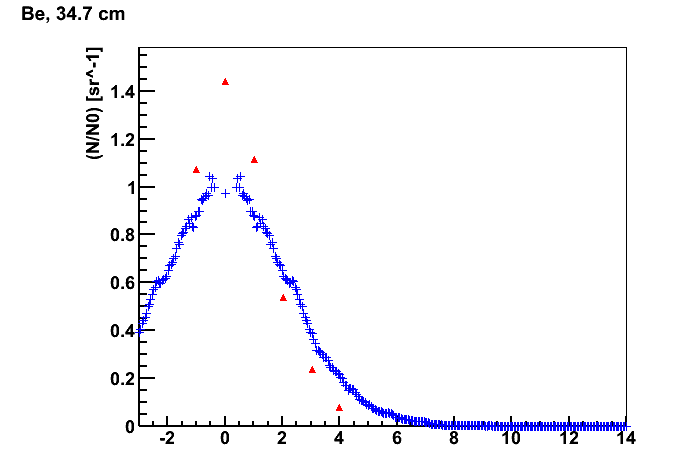
\includegraphics[width=0.45\textwidth]{images/plots/angularDistributions/AD_347_4_N.png}
\label{fig:D_43.7_4_N}
}
\label{fig:subfigureExample}
\caption[Optional caption for list of figures]{Angular distribution of beryllium fragments.}
\end{figure}
\clearpage
\subsection{Boron}
\begin{figure}[!ht]
\centering
\subfigure[5.1cm]{
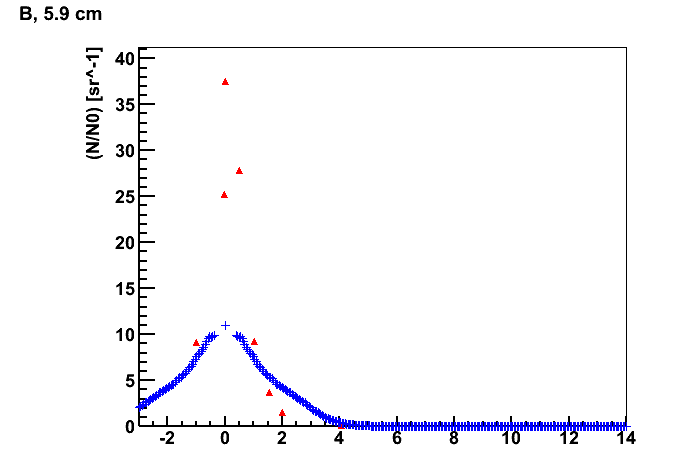
\includegraphics[width=0.45\textwidth]{images/plots/angularDistributions/AD_59_5_N.png}
\label{fig:AD_5.9_5_N}
}
\subfigure[15.1cm]{
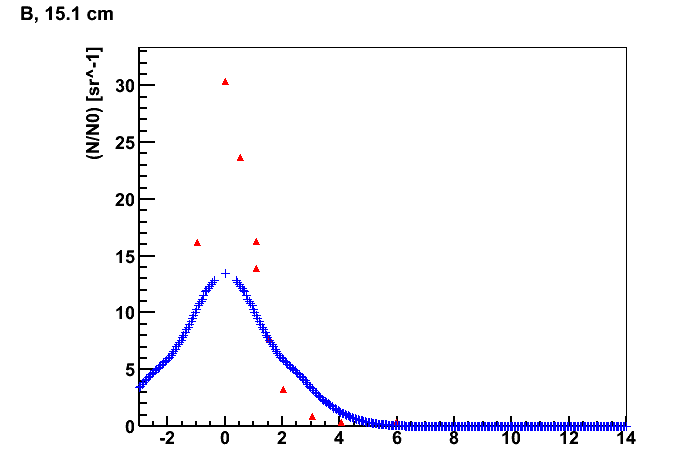
\includegraphics[width=0.45\textwidth]{images/plots/angularDistributions/AD_159_5_N.png}
\label{fig:AD_15.9_5_N}
}
\subfigure[27.1cm]{
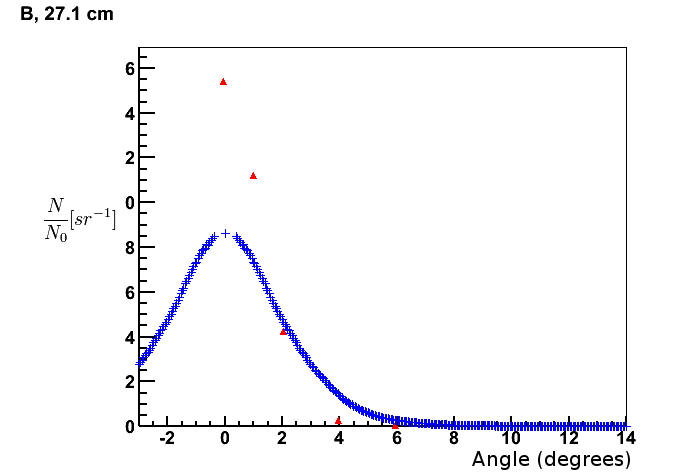
\includegraphics[width=0.45\textwidth]{images/plots/angularDistributions/AD_279_5_N.png}
\label{fig:AD_27.9_5_N}
}
\subfigure[30.4~cm]{
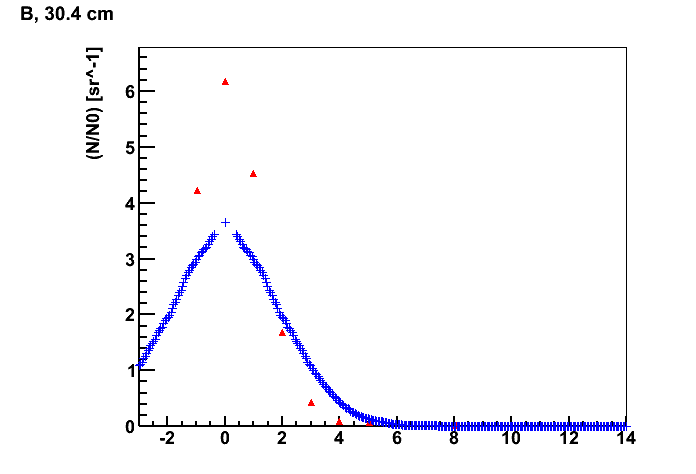
\includegraphics[width=0.45\textwidth]{images/plots/angularDistributions/AD_312_5_N.png}
\label{fig:D_31.2_5_N}
}
\subfigure[33.9~cm]{
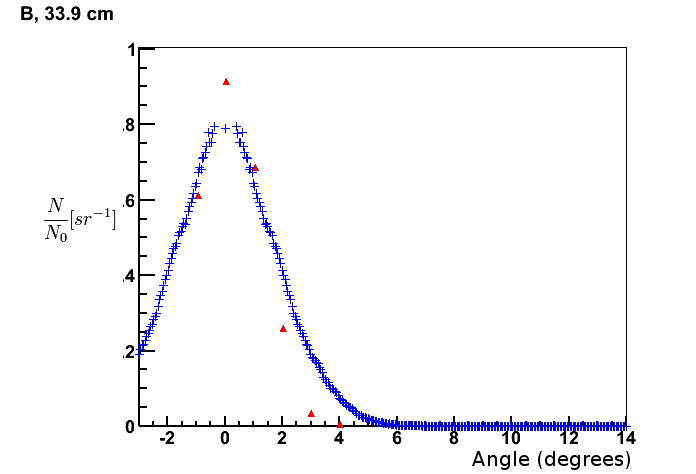
\includegraphics[width=0.45\textwidth]{images/plots/angularDistributions/AD_347_5_N.png}
\label{fig:D_34.7_5_N}
}
\label{fig:BoronAD}
\caption[Optional caption for list of figures]{Angular distribution of boron fragments.}
\end{figure}
\clearpage

%\addcontentsline{toc}{section}{Appendix B: Fragment yields for 0$^{\circ}$-10$^{\circ}$ angles}

%% Liitteiden kaavat, taulukot ja kuvat numeroidaan omana kokonaisuutenaan
\renewcommand{\theequation}{B\arabic{equation}}
\setcounter{equation}{0}  
\renewcommand{\thefigure}{B\arabic{figure}}
\setcounter{figure}{0}
\renewcommand{\thetable}{B\arabic{table}}
\setcounter{table}{0}
\renewcommand\thesection{B}
\setcounter{section}{1}
\setcounter{subsection}{0}
\section{\label{AppendixB}: Fragment yields for 0$^{\circ}$-10$^{\circ}$ angles}


\begin{figure}[!ht]
\centering
\subfigure[Hydrogen]{
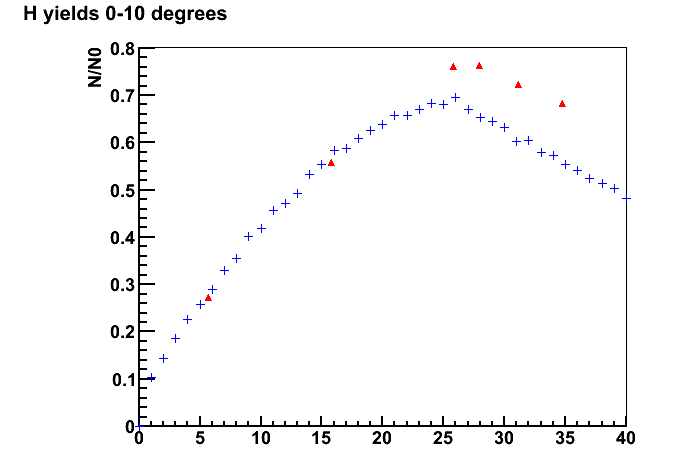
\includegraphics[width=0.45\textwidth]{images/plots/yields/fragmentYieldsForH.png}
\label{fig:fragmentYieldsForH}
}
\subfigure[Helium]{
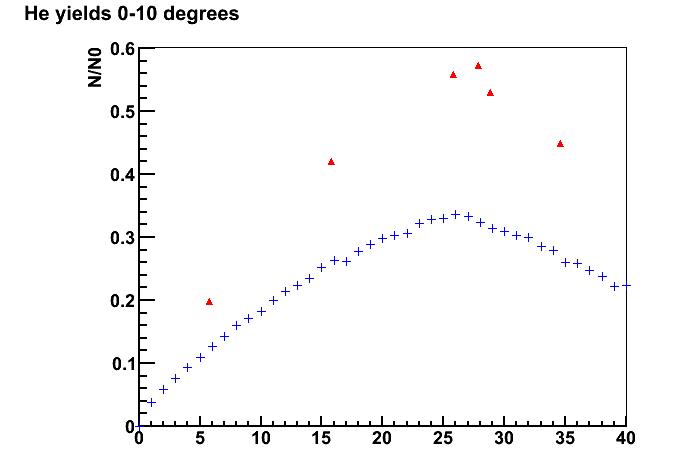
\includegraphics[width=0.45\textwidth]{images/plots/yields/fragmentYieldsForHe.png}
\label{fig:fragmentYieldsForHe}
}
\subfigure[Lithium]{
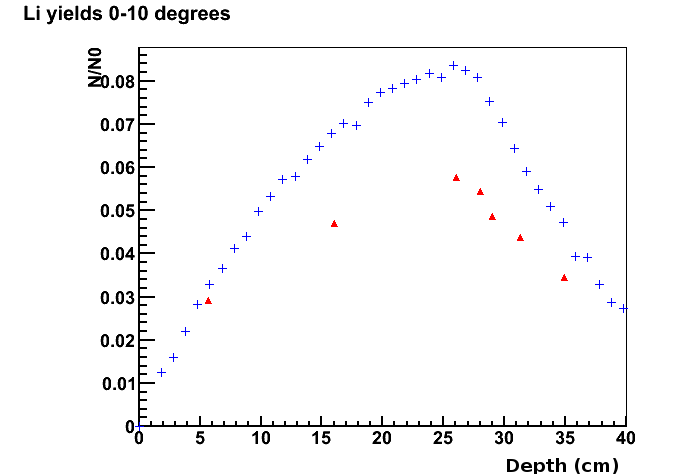
\includegraphics[width=0.45\textwidth]{images/plots/yields/fragmentYieldsForLi.png}
\label{fig:fragmentYieldsForLi}
}
\subfigure[Beryllium]{
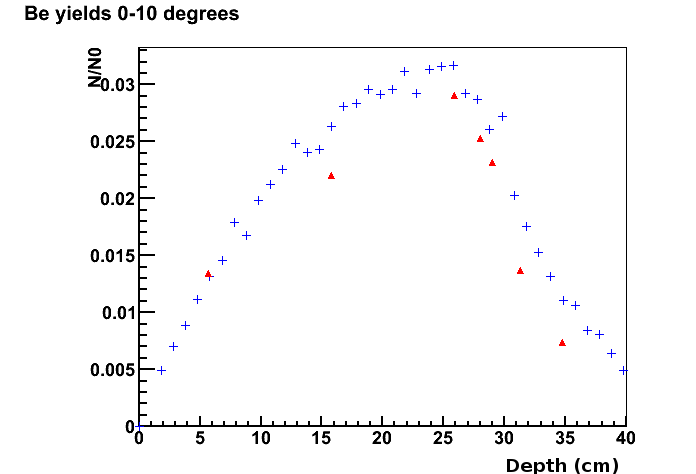
\includegraphics[width=0.45\textwidth]{images/plots/yields/fragmentYieldsForBe.png}
\label{fig:fragmentYieldsForBe}
}
\subfigure[Boron]{
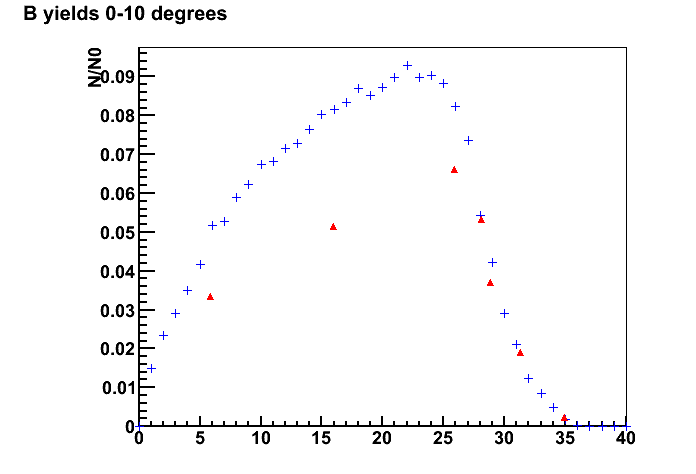
\includegraphics[width=0.45\textwidth]{images/plots/yields/fragmentYieldsForB.png}
\label{fig:fragmentYieldsForB}
}
\subfigure[Carbon]{
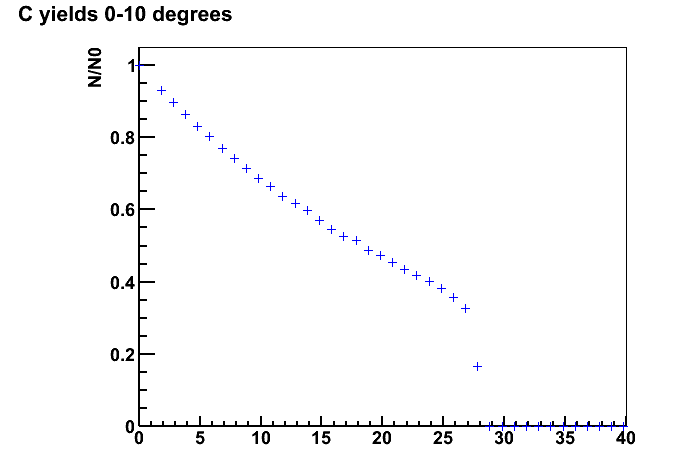
\includegraphics[width=0.45\textwidth]{images/plots/yields/fragmentYieldsForC.png}
\label{fig:fragmentYieldsForC}
}
\label{fig:fragmentYieldsZeroToTenDegrees}
\caption[Optional caption for list of figures]{Fragment yields for 0$^{\circ}$-10$^{\circ}$ angles. Match is fair with experimental data. Especially when considering the rather large error margins for heavyer fragments given by Haettner.}
\end{figure}

\clearpage
%\addcontentsline{toc}{section}{Appendix C: Future work with alternative simulation models}
%% Liitteiden kaavat, taulukot ja kuvat numeroidaan omana kokonaisuutenaan
\renewcommand{\theequation}{C\arabic{equation}}
\setcounter{equation}{0}  
\renewcommand{\thefigure}{C\arabic{figure}}
\setcounter{figure}{0}
\renewcommand{\thetable}{C\arabic{table}}
\setcounter{table}{0}
\renewcommand{\thesection}{C}
\setcounter{section}{1}
\setcounter{subsection}{0}
%\section{Future work with alternative simulation models \label{appendixincltheory}}
\section{\label{appendixincltheory}: Future work with alternative simulation models}

INCL4 is a Monte Carlo type Intranuclear Cascade Model, whereas ABLA is the the complementing Monte Carlo evaporation/fission model. In practice this means INCL is used to determine what happends just after the the projectile particle hits the target nucleus, while ABLA is used to determine what nuclear process is caused through the following excitation of the target due to the collision event. It is notable that the time-frame for evaporation and fission events are orders of magnitude greater compared to the events modelled by INCL.

\subsection{INCL}

INCL is a implementation of the Liège INC model. It is designed for use in the 200~MeV-2~GeV region where standard cross-section libraries no longer are sufficient. Containing only few free parameters INCL has proven predictive power.

INCL is called into action when Geant4 selects from available model an inelastic collision will take place. INCL then takes as parameters the beam-particle and the target nucleus. It then proceeds to randomly pick what type of collision will happen by selecting the impact parameter between zero and the the target nucleus radius. The impact parameter is defined as the perpendicular distance between the velocity of the projectile and the center of the nucleus it is approaching.

In the Liège INC model particles move in straight deterministic trajectories, which makes upcoming collisions practical to predict in the INCL code.
 The nucleus in INCL is modelled as Fermi-gas in a Woods-Saxon potential. %fixme woods-Saxon
 The Woods-Saxon potential barrier gives a potential barrier that is smooth. Thus, in the INCL code the nucleons are randomly picked from a Woods-Saxon probability density distribution.

\begin{equation}
\rho(r) = \begin{cases}
\frac{\rho_{0}}{1+\exp({\frac{r-R}{a}})} & 0 < r < R \\
0 & \text{otherwise}
\end{cases}
\label{WoodsSaxonINCL}
\end{equation}

If the energy of the bullet particle breaks the nucleus potential barrier and enters the nucleus several binary collisions between participating nucleons will take place, smaller particles may be emerge out from the nucleus. Spectator particles may move around the nucleus and bounce off its edges by reflection, however, they will not leave the nucleus.

The kinetics of the model are bound by the physical laws of conservation of baryon number, charge, energy, momentum and angular momentum and respect the Pauli blocking principle. Furthermore, pion-production is governed through the relation of $NN \rightleftharpoons N \Delta, \Delta \rightleftharpoons N\pi$ (with a stochastically determined mass for $\Delta$).

The major free parameter of the INCL code is the stopping-time; the time before thermal equilibrium can be assumed and thus the process handed over to the evaporation and fission phase. The INCL code has chosen the stopping time as a suitable function of the target nucleus size so that $$t_{stop} = f_{stop}t_{0}(\frac{A_T}{208})^{0.16},$$ where $f_{stop} = 1.0$. The stopping-time of INCL4 is considerably longer than for many models where discrete potential barriers are defined for the nucleus.

A further discussion of the theoretical basis of the Liège INC model and INCL code is available in references ~\cite{PhysRevC.66.044615,iia}.

\begin{figure}[ht]
\begin{center}
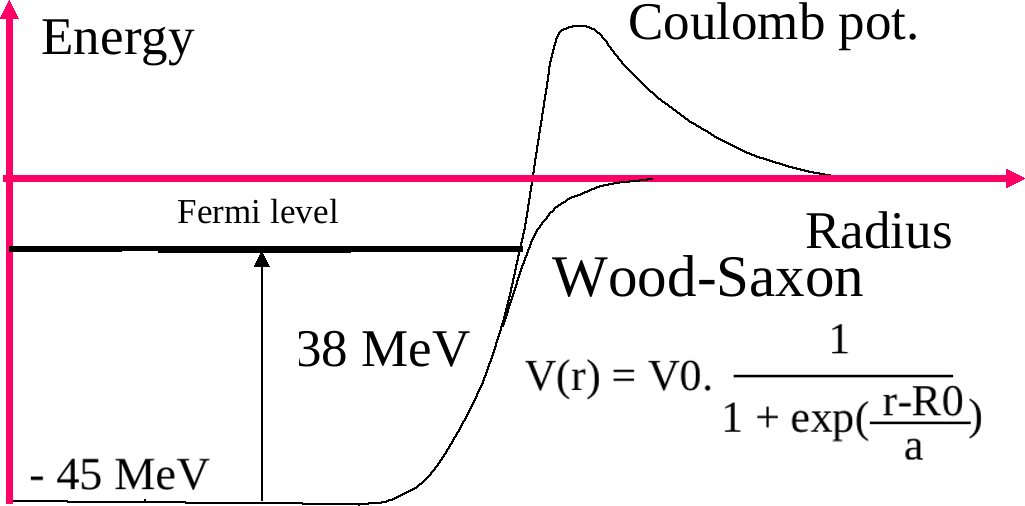
\includegraphics[width=0.6\textwidth]{images/inclPotential.png}  
\caption{\label{fig:inclpotential} Schematic of the potential model used by the INCL-model.}
 
 \end{center}
 \end{figure}


\subsection{ABLA}

The ABLA code has been developed at the GSI facility in Darmstadt, Germany. Its principal developers being K-H.~Schmidt and A.~Kelic. It is a Monte Carlo code based on a data-set {\tt G4ABLADATA} distributed alongside the code. ABLA takes as input nucleus parameters, excitation energy, mass number, charge number and nucleus spin. It then calculates on the basis of this data the probabilities for different fission or evaporation events taking place according to statistical distributions obtained from experiments and phenomenology.

ABLA comes with two different fission models SimFis3 and SimFis18. These models are based on the proven PROFI-model also developed at GSI Darmstadt. ABLA selects between competitive fission and evaporation processes as described in the flowchart~\ref{fig:ablatable}.

\begin{figure}[h] 
\begin{center}
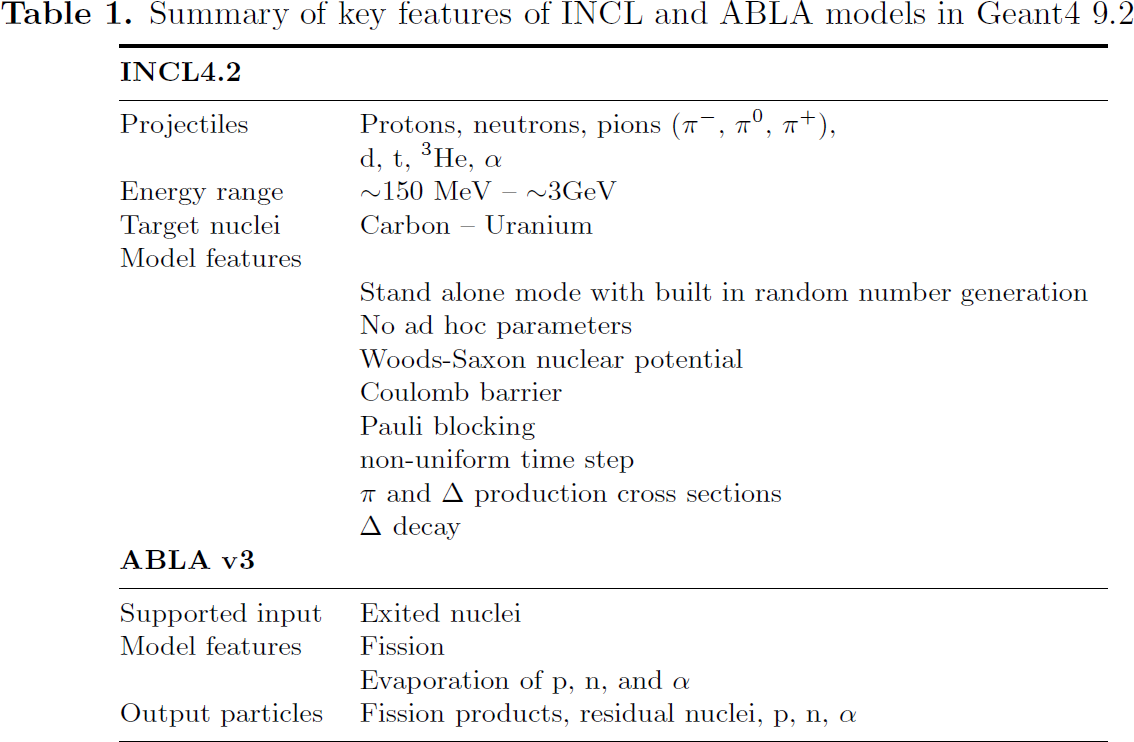
\includegraphics[width=1\textwidth]{images/inclSummary.png}  
\caption{\label{fig:inclpotential}}
 
 \end{center}
 \end{figure}

%fixme, add another picture with data

\begin{figure}[h] 
\begin{center}
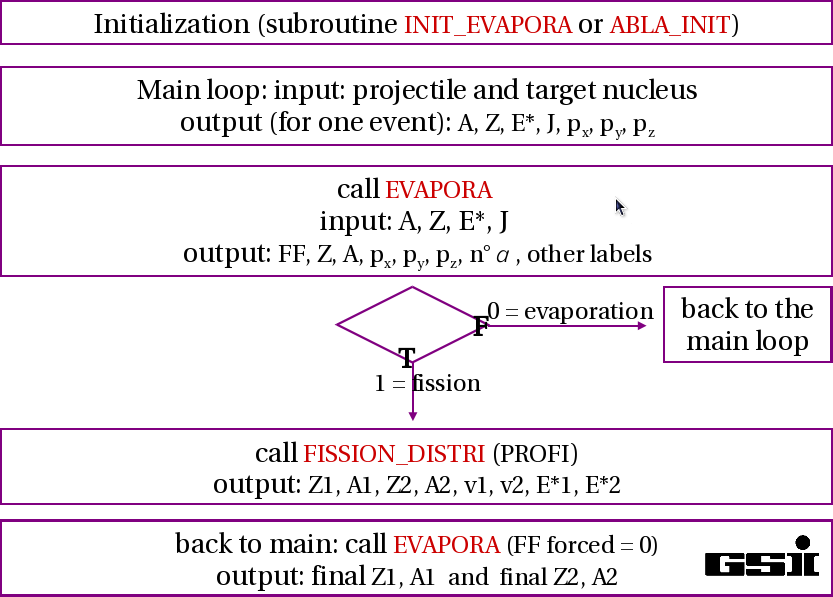
\includegraphics[width=0.6\textwidth]{images/AblaTable.png}  
\caption{\label{fig:ablatable} General flow of ABLA submodels.}
 
 \end{center}
 \end{figure}
\begin{figure}[h] 
\begin{center}
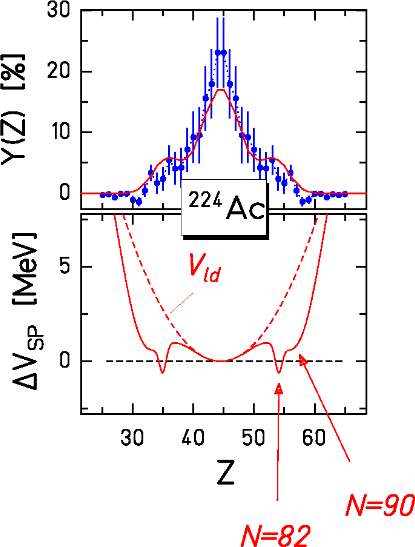
\includegraphics[width=0.3\textwidth]{images/AblaHumps.png}  
\caption{\label{fig:ablahumps} ABLA symmetric (solid line) and antisymmetric (dashed line) fission plots.}
 
 \end{center}
 \end{figure}

A further discussion of the theoretical basis of the ABLA code is available in references ~\cite{ablatalk,iia}.
%fixme add another ABLAsource

\clearpage

%\addcontentsline{toc}{section}{Appendix D: Improving usability through messenger macro commands}

%% Liitteiden kaavat, taulukot ja kuvat numeroidaan omana kokonaisuutenaan
\renewcommand{\theequation}{D\arabic{equation}}
\setcounter{equation}{0}  
\renewcommand{\thefigure}{D\arabic{figure}}
\setcounter{figure}{0}
\renewcommand{\thetable}{D\arabic{table}}
\setcounter{table}{0}
\renewcommand{\thesection}{D}
\setcounter{section}{1}
\section{\label{AppendixD}: Improving usability through messenger macro commands}

The first action task taken in this work was to implement means to speed up the use of the analysis model by means of messenger macro commands that would let the user change geometry setup inbetween runs without needing to compile the entire simulation again.

Macro commands are interpreted by the code, and are sent to the simulation and Geant4 through a specific messenger class. The features implemented through macro commands were
\begin{itemize}
 \item Ability to run multiple runs in one macro file, so that output is saved in separate root-files.
\item Ability to change the thickness of the water phantom, in such a way that all other parts of the geometry are changed as well to accustom the new phantom.
\item Ability to control the scoring area in the phantom and what is scored through command-based scoring.
\end{itemize}


So as aen example the user can give a command according to the following syntax.
\scriptsize
\begin{verbatim}
/analysis/setFileName <user-defined name>.root
\end{verbatim}
\normalsize

The implementation was done by creating an analysismessenger inheriting functionality from \textit{G4UImessenger}. An object of the type \textit{HadrontehrapyAnalysisMessenger} was created in the \textit{AnalysisManager}.


\scriptsize
\begin{verbatim}
class HadrontherapyAnalysisFileMessenger: public G4UImessenger
{
  public:
    HadrontherapyAnalysisFileMessenger(HadrontherapyAnalysisManager*);
   ~HadrontherapyAnalysisFileMessenger();
    
    void SetNewValue(G4UIcommand*, G4String);
    
  private:
    HadrontherapyAnalysisManager* AnalysisManager;
\end{verbatim}
\normalsize
\begin{figure}[h] 
\begin{center}
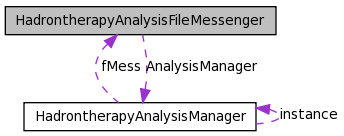
\includegraphics[width=0.3\textwidth]{images/setFileNameMessenger_1.png}  
\includegraphics[width=0.7\textwidth]{images/setFileNameMessenger_2.png}  
\caption{\label{fig:messengerUML} UML diagrams for messen ger class}
 
 \end{center}
 \end{figure}

\end{document}



